% This is a template for use with the MSU Thesis class
% Version 3.6 2022/08/23
%
% Class options: 
%[PhD]	Doctor of Philosophy (default) 
%[DEd]	Doctor of Education
%[DMA]	Doctor of Musical Arts
%[DNP]	Doctor of Nursing Practice
%[MA]	Master of Arts
%[MS]	Master of Science
%[MAT]	Master of Arts for Teachers
%[MBA]	Master of Business Administration
%[MFA]	Master of Fine Arts
%[MIPS]	Master of International Planning Studies
%[MHRL]	Master of Human Resources and Labor Relations 
%[MMus]	Master of Music
%[MPH]	Master of Public Health
%[MPP]	Master of Public Policy
%[MSW]	Master of Social Work
%[MURP]	Master in Urban and Regional Planning 
%%
% Default is PhD
%
%
% This template has everything in the right order.
% Just add real content and you're done!
%
\documentclass[]{msu-thesis}
%
% for a prettier, but possibly non-compliant table of contents use the [mixedtoc] option
% for a plain table of contents use the [plaintoc] option
% for a horrendous looking, but possibly required table of contents, use the [boldtoc] option
%
% If you have large tables/figures that need to be in landscape mode, add the [lscape] option
%
% The class accepts 12pt, 11pt or 10pt font size options. 
% For Times New Roman as in this example document, use 12pt (default).
%
\usepackage{amsmath}
\usepackage{csquotes}
\usepackage{float}
\usepackage{hyperref}
% \usepackage[document]{ragged2e}
\usepackage{graphicx}
\usepackage{caption}
\usepackage{subcaption}
%\usepackage{multirow,ragged2e}
%\usepackage{ragged2e}
\usepackage{tikz-cd}
\usepackage[final]{pdfpages}
\usepackage[
backend=biber,
style=numeric-comp,
sorting=none
]{biblatex}
\addbibresource{bibliography.bib}
% If you require per-chapter appendices add the [chapterapp] option
%
% If you require per-chapter bibliographies add the [chapterbib] option
%
% This is standard fontenc for pdflatex
% If you use LuaLaTeX or XeLaTeX you should replace this with the fontspec package
\usepackage[T1]{fontenc}
%
% If the thesis office requires Times, we'll give them Times
% You can experiment with other font packages here if you like.
% If you are using XeLaTeX or LuaLaTeX load  TeX Gyre Termes, Times or Times New Roman font with \setmainfont
\usepackage{newtxtext,newtxmath} 
%
% Load any extra packages here
%
% You must specify the title of your thesis, your name, the field of study (not department), and the year
\title{Resonance Compensation Studies at the FNAL Recycler Ring}
\author{Cristhian Gonzalez-Ortiz}
\fieldofstudy{Physics} % This should be in sentence case
\date{2024}

% If you want a dedication page, specify the text of the dedication here and uncomment the next command.
%
%\dedication{This thesis is dedicated to someone.}
%
\begin{document}

% All the stuff before your actual chapters is called the front matter
\frontmatter
% First make the title page
\maketitlepage

% if you have public abstract (optional) it should go here
%\begin{publicabstract}
% Public abstract goes here
%\end{publicabstract}

% Next make the regular abstract (obligatory)
\begin{abstract}
% Your abstract goes here.  Master's 1 page max. PhD 2 page max.
Circular accelerators, such as the ones in the Fermilab Accelerator Complex, are indispensable tools driving scientific discovery by propelling particles to high energies and high intensities. In the context of the Proton Improvement Plan II (PIP-II) at Fermilab, the Recycler Ring (RR) is confronted with the challenge of high-intensity operation. The space charge tune shifts at these intensities necessitate the mitigation of third-order resonances. By measuring the Resonance Driving Terms (RDTs) for each resonance line, their strengths and damaging effects can be quantified. 

The study is focused on the utilization of dedicated normal and skew sextupoles for the compensation of these resonance lines. By employing the response matrix method to measure the Resonance Driving Terms (RDTs) relative to the currents in these sextupoles, a methodical approach to simultaneously compensate individual and multiple third-order resonances has been developed and assessed. The assessment and verification incorporate mapping out beam losses through dynamic and static tune scans, along with the utilization of the Ion Profile Monitor (IPM) system for beam size measurements. 

Furthermore, optimization algorithms have been explored and incorporated into the resonance compensation scheme. Parallel, to the work done at Fermilab, the study extends its scope by performing related experiments at the CERN Proton Synchrotron Booster (PSB). For these experiments, multiple resonance lines in the tune diagram were compensated by optimizing the currents in the compensation elements with the aid of advanced optimization algorithms.  

High-intensity operation of the Recycler Ring involves understanding the interplay between the space charge tune spread, resonance lines, and specialized subsystems such as transverse dampers. The following study also delves into experiments that try to discern each of these phenomena, while highlighting challenges still ahead. Overall, these studies indicate the feasibility of compensating for multiple third-order resonances, contributing to the objectives of PIP-II for the reliable delivery of a 1.2 MW proton beam to experimental facilities.
\end{abstract}

% Force a newpage
\clearpage
% Make the copyright page. The Graduate School ridiculously claims that you
% can't have a copyright page unless you pay ProQuest to register the copyright.
% This is simply not the case, so put in your copyright page whether or not you
% intend to pay Proquest to register the copyright.
% Furthermore, they have occasionally complained that the copyright mark is aligned
% to the right, even though that has been the format for more than a decade.
% If they want the copyright mark aligned to the left, use \makecopyrightpage* instead. 

\makecopyrightpage 

% If you have a dedication page, uncomment the next command to print the dedication page
%
%\makededicationpage
%
\clearpage
% Your Acknowledgements are formatted like a chapter, but with no number
\chapter*{Acknowledgements}
\DoubleSpacing % Acknowledgements should be double spaced
I would like to acknowledge Dr. Robert Ainsworth for taking those couple of nutmegs when we played footy together. Thank you, Rob, for making me a better scientist and teaching me so many valuable life lessons. Thank you for always having my back.

I would like to acknowledge the instrumental role of Dr. Peter Ostroumov in these years of my Ph.D. at Michigan State University. Thank you, Peter, for pushing me to be a better physicist and scientist, every day. Thank you for believing in me, even in the moments I didn't believe in myself.

Thank you to the members of my doctoral committee, Steve Lund, Yue Hao, Paul Gueye and Kendall Mahn. I truly value every comment and every word of encouragement at all of our meetings. We did not meet frequently, but your guidance was crucial through this process. Also thank you to whole support network at MSU and FRIB---these are institutions where you will never feel alone and always have someone support you when needed.

I would like to acknowledge the whole MI/RR department at Fermilab. Thank you, Kyle, Adam, Nino, Osama, Betiay, Denton, Marty, Mike, Phil, MaryKate, Matilda and Meiqin, and whoever I might have left out. Thank you for having the patience and your unconditional support while I pushed through with my experiments. You guys always had a smile even when I asked the most basic questions. Special acknowledgement to the operations team at Fermilab for always being open to questions and discussion. Thank you for having the patience to withstand me when I would continuously trip the permit on beam losses. I would also like to acknowledge the hospitality and awesomeness of our CERN collaborators, specially Foteini and Tirsi. 

Luisa. Tú has sido el soporte y la inspiración estos últimos años para poder estar a puertas de cruzar la meta. Gracias por siempre estar ahí y no rendirte nunca con lo nuestro. Vamos a lograr grandes cosas juntos. Ya casi adoptamos un perrito, manguitos szah.

Gracias a toda mi familia, incluyendo a esos amigos que considero mi familia, por apoyarme en este camino. Desde Bogotá hasta llegar a Chicago pasando por Lansing. Nunca pensé en llegar tan lejos de la loma. No hubiera podido terminar este doctorado sin el apoyo de todos ustedes. Gracias por estar ahí en cada momento de mi vida. Thank you, Sjuju, the great celestial whale overseer.

%
\clearpage
% We need to turn single spacing back on for the contents/figures/tables lists
\SingleSpacing
\tableofcontents* % table of contents will not be listed in the TOC
%\clearpage
%\listoftables % comment this out if you have no tables
%\clearpage
%\listoffigures % comment this out if you have no figures
%
% If you have a Key to  Abbreviations/symbols you would add each abbreviation in its display order
% using as in the following examples:
\abbrev{MSU}{Michigan State University}
\abbrev{FNAL}{Fermilab National Accelerator Laboratory}
\abbrev{RR}{Recycler Ring}
\abbrev{MI}{Main Injector}
\abbrev{RDTs}{Resonance Driving Terms}
\abbrev{NuMI}{Neutrinos at the Main Injector}
\abbrev{PSB}{CERN Proton Synchrotron Booster}
\abbrev{ACNET}{Accelerator Control Network}
\abbrev{TbT}{Turn-by-Turn Data}
\abbrev{NAFF}{Numerical Analysis of Fundamental Frequencies}
\abbrev{GFCs}{Generating Function Coefficients}
% Then issue a \clearpage and print the list 
\clearpage
\listofabbreviations 
% Comment out the code above if you have no abbreviations
% See the documentation if you need to change the width or format of the abbreviation column

% See the class documentation and the Memoir manual for how to create other lists
%
% If you are using an algorithm formatting package (e.g. algorithmicx or algorithm2e)
% please read the class documentation carefully on how to use these packages with the class
% The class provides an {algorithm} environment and a \listofalgorithms by default 
%
\mainmatter
%
% The next line removes the dots in chapter headings in the TOC
% May violate thesis office rules
%\addtocontents{toc}{\protect\renewcommand{\protect\cftchapterdotsep} {\cftnodots}}

% ALL documents using this class must have \chapter divisions
% If you are using it for an MA/MS thesis you still need to have chapters, even if they are very small.
\chapter{Introduction}
\label{sec:ch1}
 
Particle accelerators are the workhorses for modern scientific discoveries. Experimental nuclear and particle physics research benefit greatly from the progress of accelerator physics and technology. Accelerator physics is a rich field of applied physics living on the intersection of electromagnetism, solid-state and atomic physics, nonlinear mechanics, plasma physics, quantum mechanics, just to name a few \cite{sylee}. Furthermore, the design and operation of modern accelerator projects require costly enterprises of scientists, engineers, operators, and politicians coming together under one single metaphorical roof. Everyone coming together to perform \textquote{megascience} \cite{fermilab1}.         

The scientific principle of particle accelerators involves the acceleration, steering and/or storage of charged particles through electromagnetic manipulations. These manipulations occur through a plethora of devices and components that can control electromagnetic fields, e.g., magnets, electrical cavities. The group of particles that is subject to this electromagnetic handling is referred to as "the beam". The field of beam dynamics studies the interaction between the beam and the steering devices, as well as the Coulomb interactions between the beam itself---this is known as space charge physics. An additional distinction can be made when these steering devices are configured in a circular or linear fashion. This gives rise to the distinction between circular accelerators and linear accelerators (Linacs).

Furthermore, particle accelerators can be categorized by the type of elementary particles that compose the beam and how close to the speed of light they are traveling. The first category refers to the distinction between hadrons and leptons---particles that interact or do not interact through the strong force, respectively \cite{griffiths}. For example, protons and heavy ions are considered hadrons, while electrons and muons are considered leptons. The second category can be summarized if particles in the machine travel at a high or low energy. An example of a low-energy hadron machine is the heavy ion Linac at FRIB (Facility for Rare Isotope Beams) \cite{frib}. An example of a high-energy lepton machine was the Stanford Linear Accelerator located at SLAC National Accelerator Laboratory \cite{slac}. The two most famous high-energy hadron machines in history are the Tevatron \cite{tevatron}, which operated at Fermilab, and the LHC (Large Hadron Collider), operating at CERN \cite{lhc}. Furthermore, there are accelerator projects that encompass several categories such as the future EIC (Electron-Ion Collider) being built at Brookhaven National Laboratory \cite{eic}, which will use an electron ring---a lepton machine---and a heavy-ion circular accelerator---a hadron machine---to probe new physics. This is just to name a few. There's a plethora of accelerator projects around the world that are either operational, under commissioning or being designed. 

The following thesis will explore the beam dynamics of a circular machine. The research results are applied to the Fermilab Recycler Ring, which is used to store high-energy protons.

\section{Circular Accelerators and Storage Rings}

As will become more apparent on Ch. \ref{sec:ch2}, a particle accelerator can be thought of as a composition of accelerator-themed LEGO® bricks \cite{forest}. Each elemental LEGO® brick can be thought of as an accelerator component performing some mapping on the charged particles entering it. As it turns out, these LEGO® bricks can be assembled together circularly to give rise to circular accelerators. The assembly of these blocks in a particular shape gives rise to what is known as the lattice of the accelerator.

The acceleration part of these structures comes from elements inside the lattice that introduce some sort of electromotive force in the longitudinal direction. The most common example for these blocks are radio-frequency (rf) cavities \cite{sylee}, with super-conducting rf cavities also as an established technology \cite{srfcavs}. Particles that go through these elements gain energy on every pass. For the case where there are no acceleration blocks on these structures, a storage ring arises. Nevertheless, storage rings can also have rf cavities just for longitudinal beam manipulation, but no overall acceleration---such is the case of the Recycler Ring.    

Circular accelerators are special due to the fact that particles have to pass thousands or even millions of turns through the same LEGO® blocks. This gives birth to very interesting and complex dynamics inside these machines. One of these phenomena are called betatron resonances. The most simple lattice of a high energy machine is composed of focusing and steering blocks, and they are dipole and quadrupole magnets, i.e. the lowest-order multipole magnets. For reasons that will become apparent in Ch. \ref{sec:ch2}, these elements, in combination with free drift spaces, represent linear blocks. For the simplest circular machine, these linear LEGO® bricks are assembled together to create a linear lattice. A linear lattice is designed to have stable particle orbits all around the accelerator. Nevertheless, accounted or unaccounted elements, described by linear or nonlinear blocks, around the machine can perturb the stable orbits. Ultimately, the effect of these perturbations can add up coherently over many turns to push the beam out of the acceptance of the lattice, i.e., the particles hit the enclosing vacuum pipe and create beam loss. This whole process is known as a betatron resonance in a circular accelerator. A mathematical description of this process is described on Ch. \ref{sec:ch2}.

The following thesis describes an effort to mitigate the deleterious effect of these resonances in the Recycler Ring. After dipole and quadrupole, the third order of multipole magnetic fields is the sextupole component. Therefore, sextupole fields around the lattice are the source of third order betatron resonances. Specifically, this thesis explores mitigation techniques to these third order resonances, mainly in the Fermilab Recycler Ring (see Ch. \ref{sec:ch3}, Ch. \ref{sec:ch4} and Ch. \ref{sec:ch6}), but also with some experiments done at the CERN Proton Synchrotron Booster (see Ch. \ref{sec:ch5}). 

\section{Fermilab}

The best introduction to Fermilab is to cite an excerpt from Ref. \cite{fermilab1}:
\begin{displayquote}
    \begin{flushleft}
    [...] A passenger peers through the window of an airplane. As his plane flies into Chicago's O'Hare Field from the west, he notices a large ring on the ground below (see Fig. \ref{fig:fermia}). Near it he sees a towering white structure, a group of colorful smaller buildings, an expanse of forest, open fields, and lakes.

    "What is that ring?" he asks his neighbor.

    "Fermilab," she replies. "It's a physics laboratory. The government supports research there into what the universe is made of."

    "Why the ring?"

    "It's the four-mile-round main ring of a machine called the Tevatron. It turns protons into tools for looking inside the atomic nucleus. Huge magnets steer the protons around the ring, while high voltages accelerate them. [...]" (pp. 1)
    \end{flushleft}
\end{displayquote}

\begin{figure}[H]
    \centering
    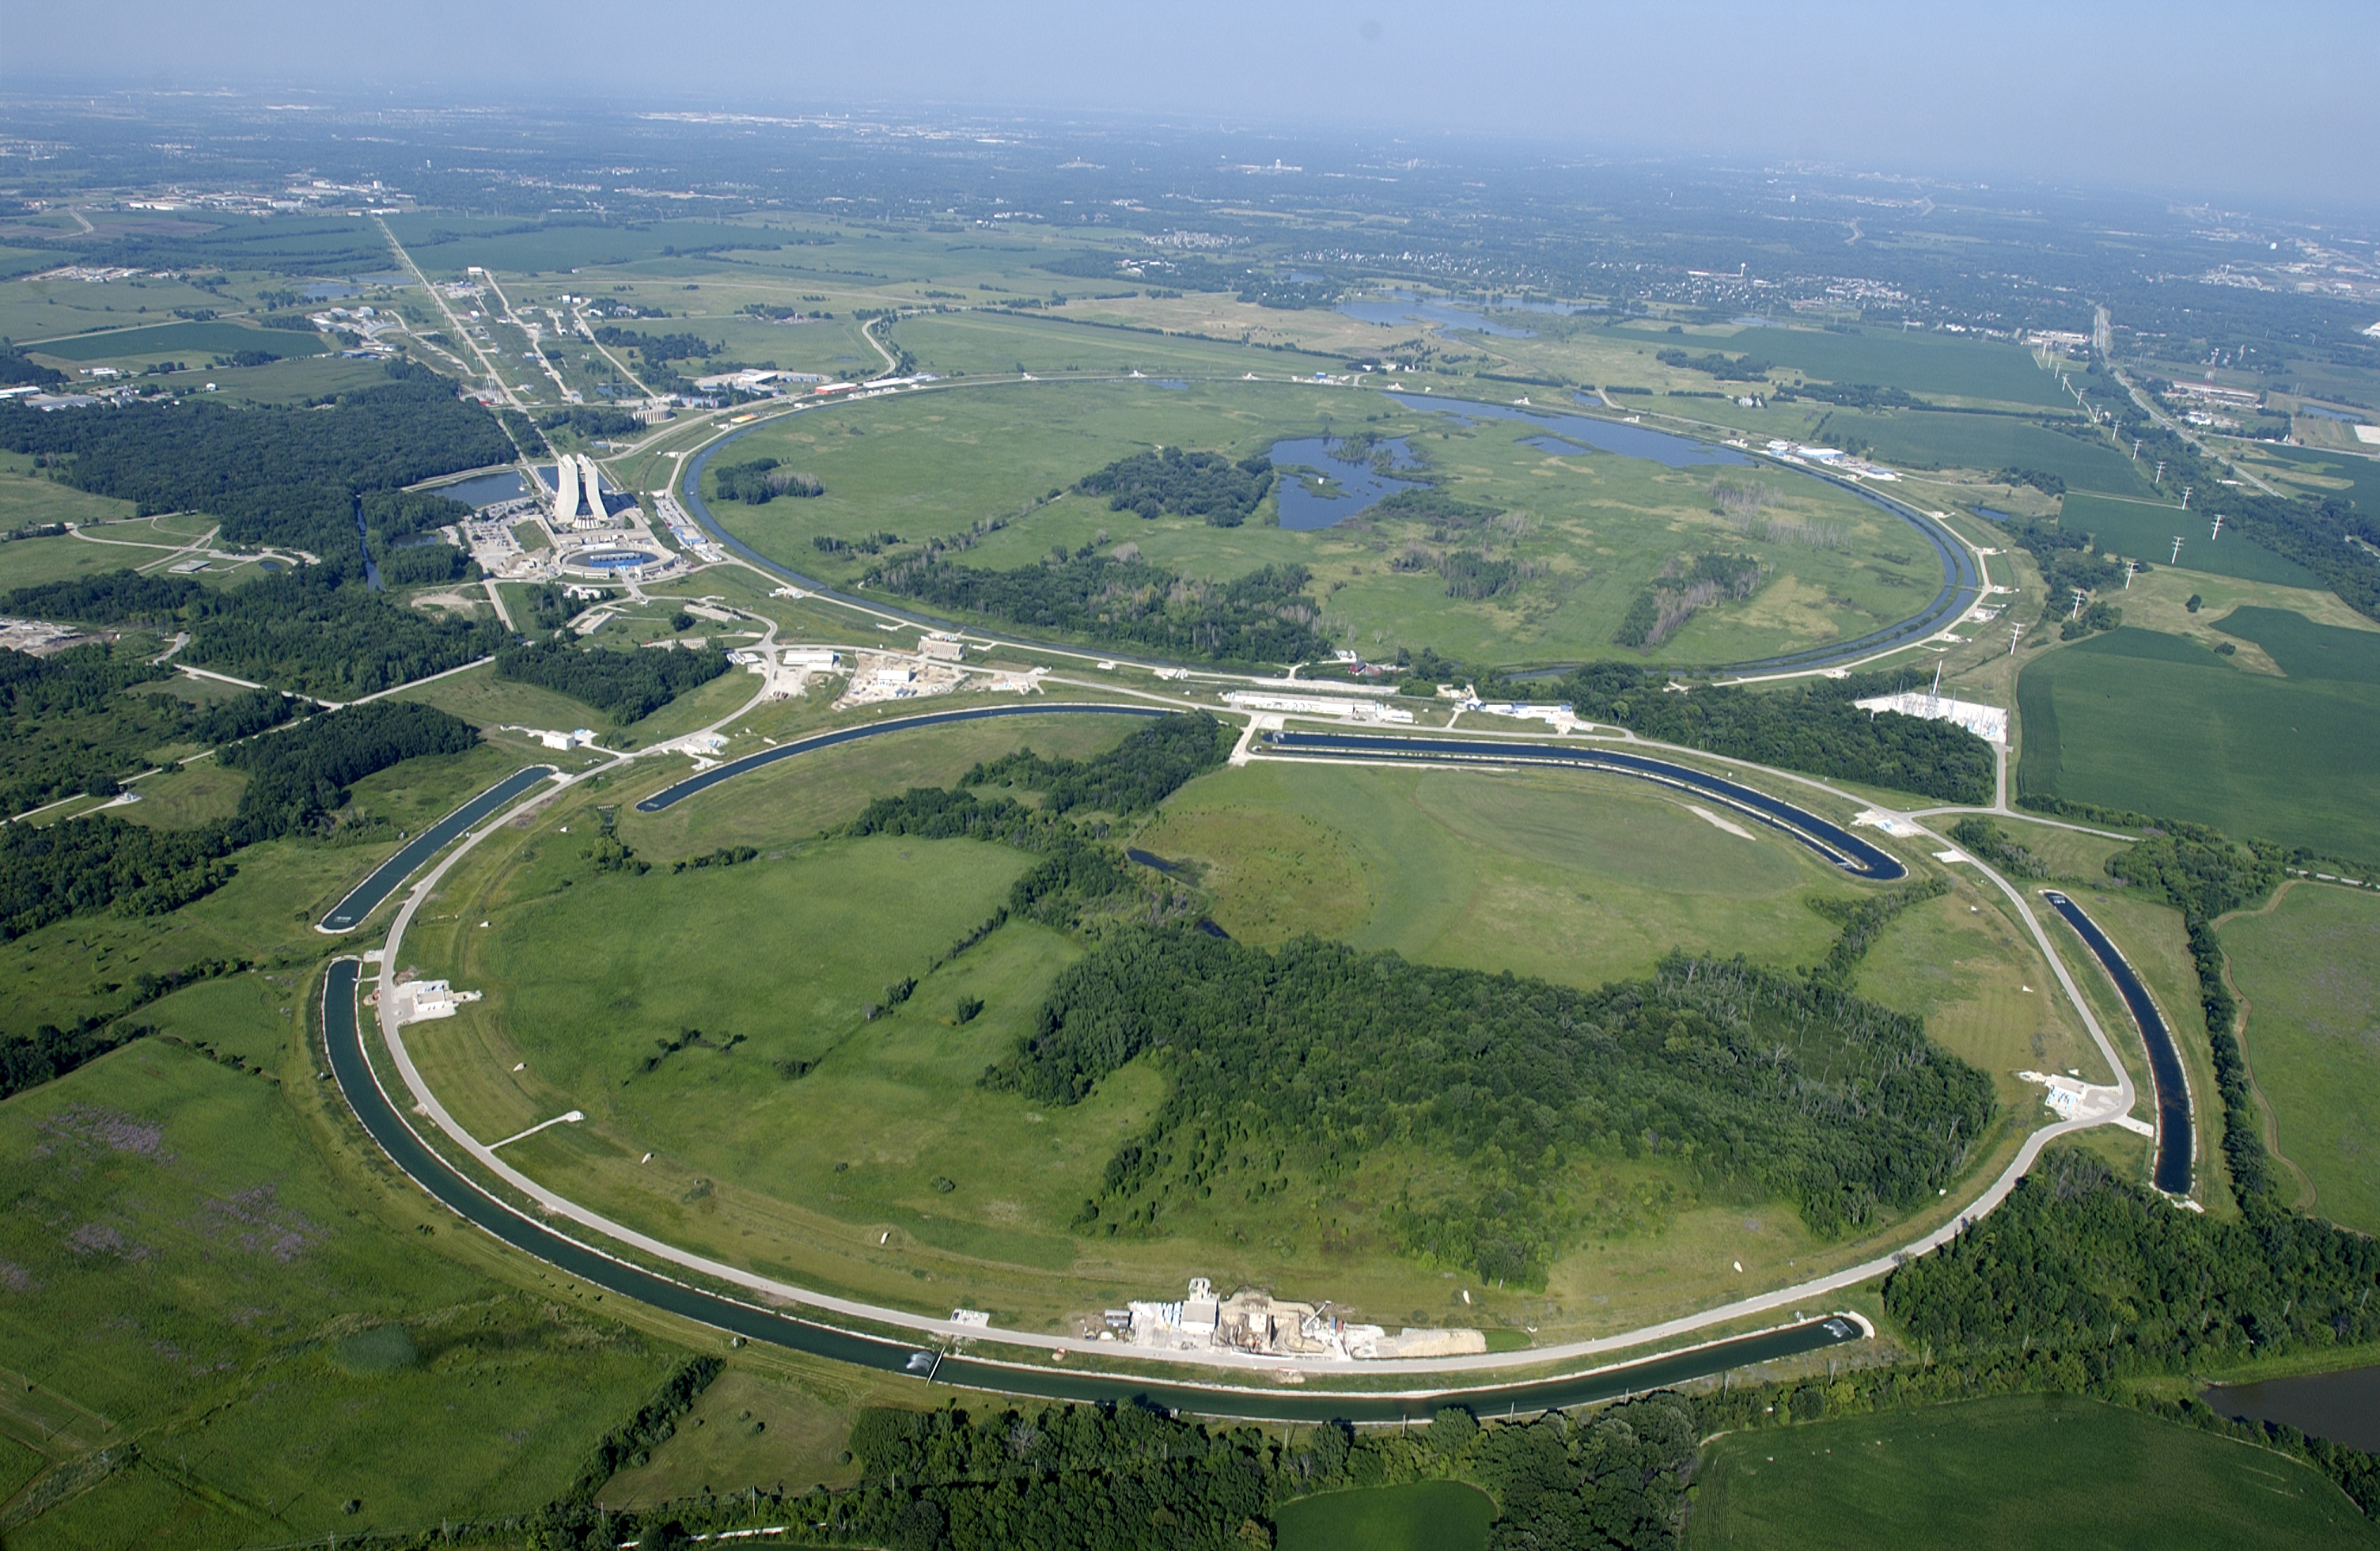
\includegraphics[width=\columnwidth]{chapter1/fermilab.jpeg}
    \caption{Aerial view of the Fermi National Accelerator Laboratory (FNAL) located in Batavia, IL, USA \cite{fermipic}.}
    \label{fig:fermia}
 \end{figure}

The Fermi National Accelerator Laboratory (FNAL), better known as Fermilab, has a long and rich history of designing, building and operating high-energy particle accelerators. Ever since the founding director of Fermilab, Robert R. Wilson, envisioned the 400 GeV Main Ring back in 1967, Fermilab has been at the forefront of accelerator physics \cite{fermilab1,fermi50,tevatron}. The most famous accelerator project hosted by Fermilab has been the Tevatron, a proton-antiproton circular collider with a circumference of around 6.28 km. This machine was injected protons and antiprotons from smaller machines, that are still in operation or have been repurposed as of 2024, e.g. the Recycler Ring. The Tevatron operated up until 2011, leaving an indelible legacy in the field of high energy and accelerator physics. Nostalgia aside, Fermilab still hosts a deluge of particle physics experiments connected to its main accelerator complex.      

The current layout of the Fermilab Accelerator Complex is summarized in Fig. \ref{fig:fac}. As of 2024, the Fermilab Accelerator Complex is composed of an $H^-$ source that connects to a linear accelerator, accelerating the ions to an energy of 400 MeV. This linear accelerator feeds to the first circular machine---the Booster---where protons are achieved and accelerated to an energy of 8 GeV. After the Booster, the protons are transported to the Recycler Ring (RR), which is the second circular machine. In the RR, protons are stacked and stored in order to increase the beam intensity delivered to the Main Injector (MI). This last circular accelerator is where protons are accelerated from an energy of 8 GeV to 120 GeV. Once at this energy, the protons are transported to the Neutrinos at the Main Injector (NuMI) experiment, in order to create the world's most intense neutrino beam \cite{numi1}. Nevertheless, all throughout the chain of accelerators, beam is also delivered to a plethora of other experiments being conducted at Fermilab. Therefore, the facility has several modes of operation depending on the experiments that are online. A more detailed and technical study of the current Fermilab Accelerator Complex, focusing on the Recycler Ring, is given on Ch. \ref{sec:ch3}.   

\begin{figure}[H]
    \centering
    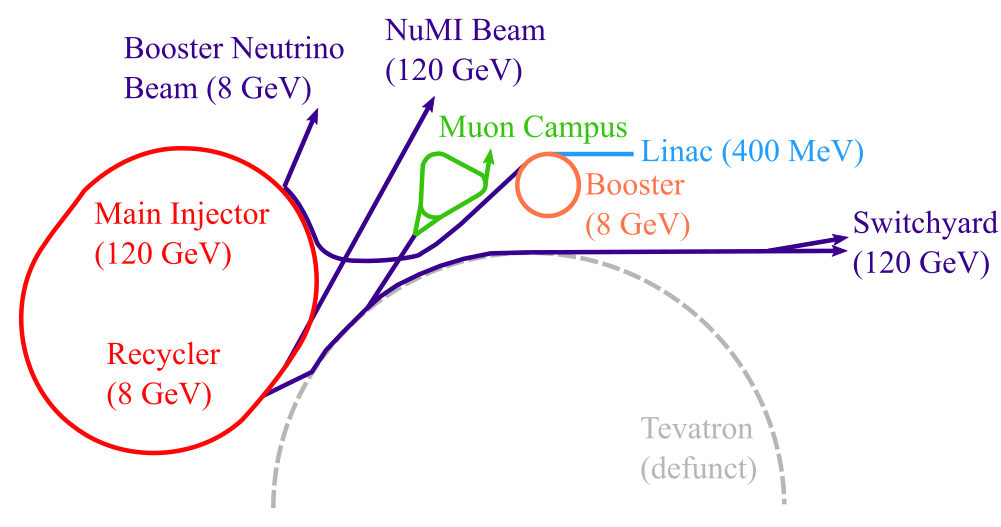
\includegraphics[width=\columnwidth]{chapter1/complex.png}
    \caption{Schematic layout of the Fermilab Accelerator Complex as of 2024. Original plot provided by R. Ainsworth, first published on Ref. \cite{rr1}.}
    \label{fig:fac}
 \end{figure}

\section{Outline}

The following thesis will explore the compensation of third-order resonances in the Fermilab Recycler Ring. \hyperref[sec:ch1]{Chapter 1} introduces the motivation behind this thesis work. \hyperref[sec:ch2]{Chapter 2} summarizes single particle dynamics with the help of exponential Lie operators and moves forward to introduce a relevant concept of collective beam dynamics: the space charge tune shift. This theoretical overview gives segue into the \hyperref[sec:ch3]{Ch. 3} of this thesis, where the Recycler Ring is introduced and described in detail. Motivation for the compensation of third order resonances is given in this chapter under the framework of current and future operation of the RR. With the basic physics concepts and the description of the machine put in place, \hyperref[sec:ch4]{Ch. 4} describes in full detail the scheme and experiments developed in order to compensate third order resonances at low intensities. Before moving to explore the Recycler Ring at high intensities, \hyperref[sec:ch5]{Ch. 5} provides an interlude in order to show a series of experiments done at the CERN PS Booster. These experiments explore the use of advanced optimization algorithms to compensate multiple resonance lines simultaneously. Coming back to Fermilab, \hyperref[sec:ch6]{Ch. 6} showcases the studies and experiments done at high intensities in the RR in order to understand the interplay between the compensation of resonance lines and space charge effects. Finally, \hyperref[sec:ch7]{Ch. 7} brings down the curtain by providing some general conclusions and future work stemming from this thesis.
\chapter{The FNAL Recycler Ring}
The Fermilab Recycler Ring (RR) is one of the circular accelerators located .

\section{General Specifications}

\section{Tune Diagram and Resonances}

\section{High Intensity and Tune Footprint}

\chapter{The FNAL Recycler Ring}
\label{sec:ch3}

\section{\label{sec:intro31}Introduction}
The Fermilab Recycler Ring (RR) is one of the circular accelerators located in the Fermilab Accelerator Complex. It was originally designed to store and accumulate antiprotons that remained from a Tevatron event \cite{rr0}. The recycling of antiprotons was deemed ineffective and was never operationally implemented \cite{rrnagaitsev}. Since 2011, the RR has been repurposed to act as a pre-injector to the Main Injector (MI) by storing and accumulating protons \cite{rr1}. It is worth pointing out, that the MI and the RR share the same tunnel, which has a circumference of 3.319 km (2.062 mi). The work done for this thesis focuses on the Recycler Ring. The following chapter starts by giving a general description for the operation and physics of the Recycler Ring. The next sections introduce and motivate the compensation of third order resonances for high intensity operation.  

The MI/RR complex is fed protons by the Proton Source, which by itself consists of the Pre-Accelerator, the Linear Accelerator (Linac), and the Booster. The Pre-Accelerator systems provide $H^-$ ions to the Linac, where they are accelerated to an energy of 400 MeV. After this, the beam is injected into the Booster Ring. The Booster is a rapid-cycling synchrotron operating at a 15 Hz repetition rate. During this injection process, the $H^-$ beam passes through a carbon stripping foil, and it incorporates to the circulating proton beam. The Booster ramps the energy up from 400 MeV to 8 GeV. This 8 GeV proton beam can either go to the Booster Neutrino Experiments or get injected into the Recycler Ring. Once in RR the beam has two possible destinations: 1) high energy neutrino experiments through MI or 2) Muon Campus. For the latter, proton beam gets rebunched from 53 MHz to 2.5 MHz and transported to Muon Campus. For high energy neutrino experiments, the proton beam gets slip-stacked, hence doubling the intensity that gets injected into Main Injector. Once in MI, the beam is accelerated to 120 GeV and sent to the NuMI (Neutrinos at the Main Injector) beam facility \cite{rr1, rrnagaitsev, numi1}. A description of the current accelerator complex is shown in figure \ref{fig:fnal}, including the experimental beamlines which feed neutrino, muon and fixed target experiments.

\begin{figure}[H]
   \centering
   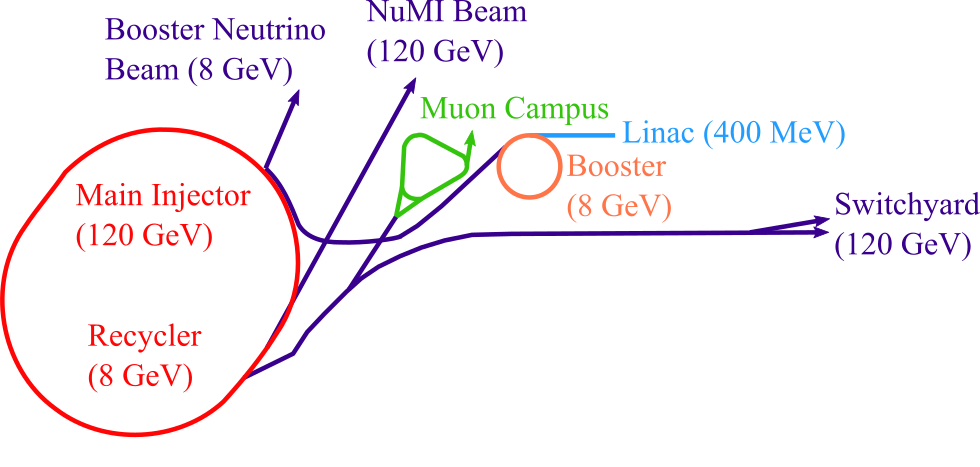
\includegraphics[width=\columnwidth]{chapter3/complex_noTev.png}
   \caption{Current operational layout of the Fermilab Accelerator Complex as of 2024. Original plot provided by R. Ainsworth, first published on Ref. \cite{rr1}, but modified for this document.}
   \label{fig:fnal}
\end{figure}

The Proton Improvement Plan II (PIP-II) is the first step in establishing the Fermilab Accelerator Complex as a multi-MW proton facility \cite{pipII1}. The near-future objective is to deliver a 1.2 MW proton beam to the Deep Underground Neutrino Experiment (DUNE) through the Long-Baseline Neutrino Facility (LBNF) \cite{dune}, still in construction. In order to meet this goal, several upgrades are being planned in the accelerator complex, including a new 800 MeV superconducting linear accelerator. The future plan for the layout of the Fermilab Accelerator Complex is shown in Fig. \ref{fig:fnalpip2}. With minimal upgrades to the Main Injector and Recycler Ring, but with a substantial overhaul of the Booster Ring, this will allow for a 50\% increase in particles per pulse intensity. Table \ref{tab:rrparams} also specifies some upgrades that will happen for the PIP-II era. Some examples include an increase of the particle per bunch intensity, a shortening of the Main Injector acceleration ramp and an increase in the Booster ramping rate. As the Recycler Ring starts to deal with higher intensities from the PIP-II upgrade, it is important to mitigate the effects of space charge as discussed in Secs. \ref{sec:resonances} and \ref{sec:sc1}. Particles along the bunch will experience space charge force leading to detuning in their betatron frequencies. Given the incoherent nature of this process, this leads to the beam having a larger tune spread in the tune diagram and having particles operate on top of resonances.

\begin{figure}[H]
   \centering
   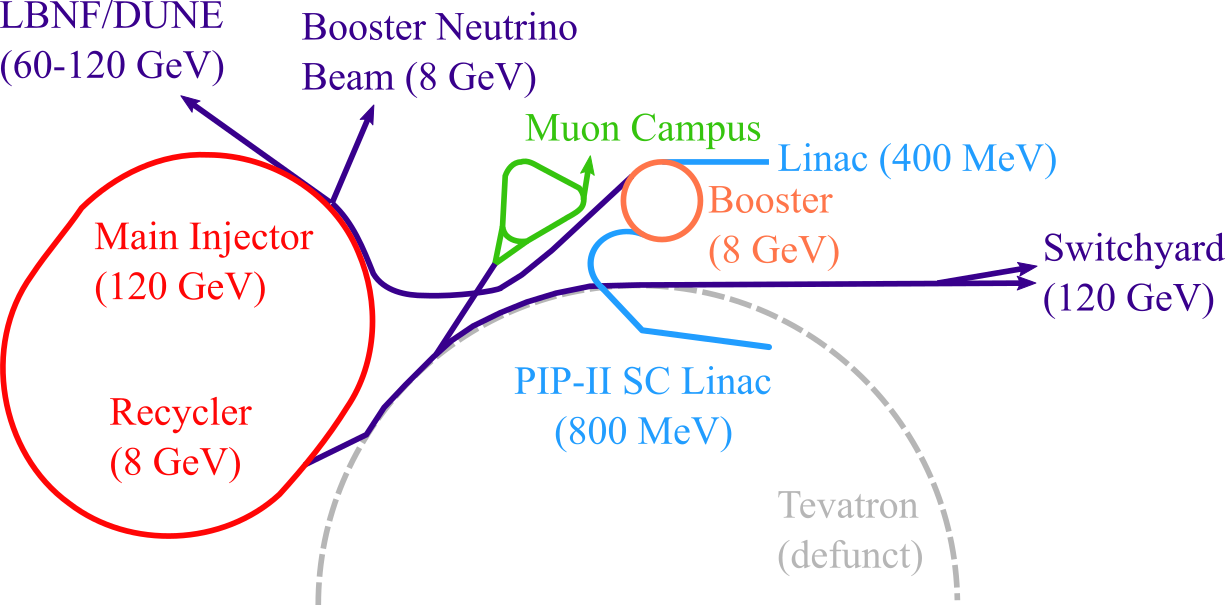
\includegraphics[width=\columnwidth]{chapter3/complexPIPII.png}
   \caption{Future layout of the Fermilab Accelerator Complex for the Proton Improvement Plan II (PIP-II). Original plot provided by R. Ainsworth, first published on Ref. \cite{rr1}, but modified for this document.}
   \label{fig:fnalpip2}
\end{figure}

\section{General Description}

The RR is a permanent magnet storage ring operating at a fixed momentum of 8.835 GeV/c equivalent to an energy of 8 GeV. The basic cell structures of this machine are FODO (Focusing Quadrupole - Drift - Defocusing Quadrupole - Drift) cells. During its conception, the need for a quick and non-expensive design spurred the idea of combining quadrupole and dipole magnets into one combined function magnet. These combined function magnets can be seen in Fig. \ref{fig:rrtunnel} as the green covered magnets on the top ring--the Recycler Ring. In order to further reduce costs and human labor during its construction, these magnets were chosen to be permanent magnets made out of a strontium ferrite \cite{rr0}. Some advantages of having permanent magnets is that there is no need for power supplies, cooling systems or power distribution cables. Consequently, these type of magnets are very stable against time and temperature. Nevertheless, the magnetic field of such magnets does degrade over time. Reference \cite{rr1} shows how the fields in RR-type magnets can degrade around 1\% after 20 years. Ultimately, this slightly changes the nominal energy in the machine. 

\begin{figure}[H]
   \centering
   \includegraphics[width=\columnwidth]{chapter3/tunnel.jpg}
   \caption{Picture of the Main Injector (blue and red magnets in the bottom) and the Recycler Ring (green magnets up top) tunnel.}
   \label{fig:rrtunnel}
\end{figure}


\cite{pipII1} \cite{rr2} \cite{fermi_rookie}

\begin{figure}[H]
   \centering
   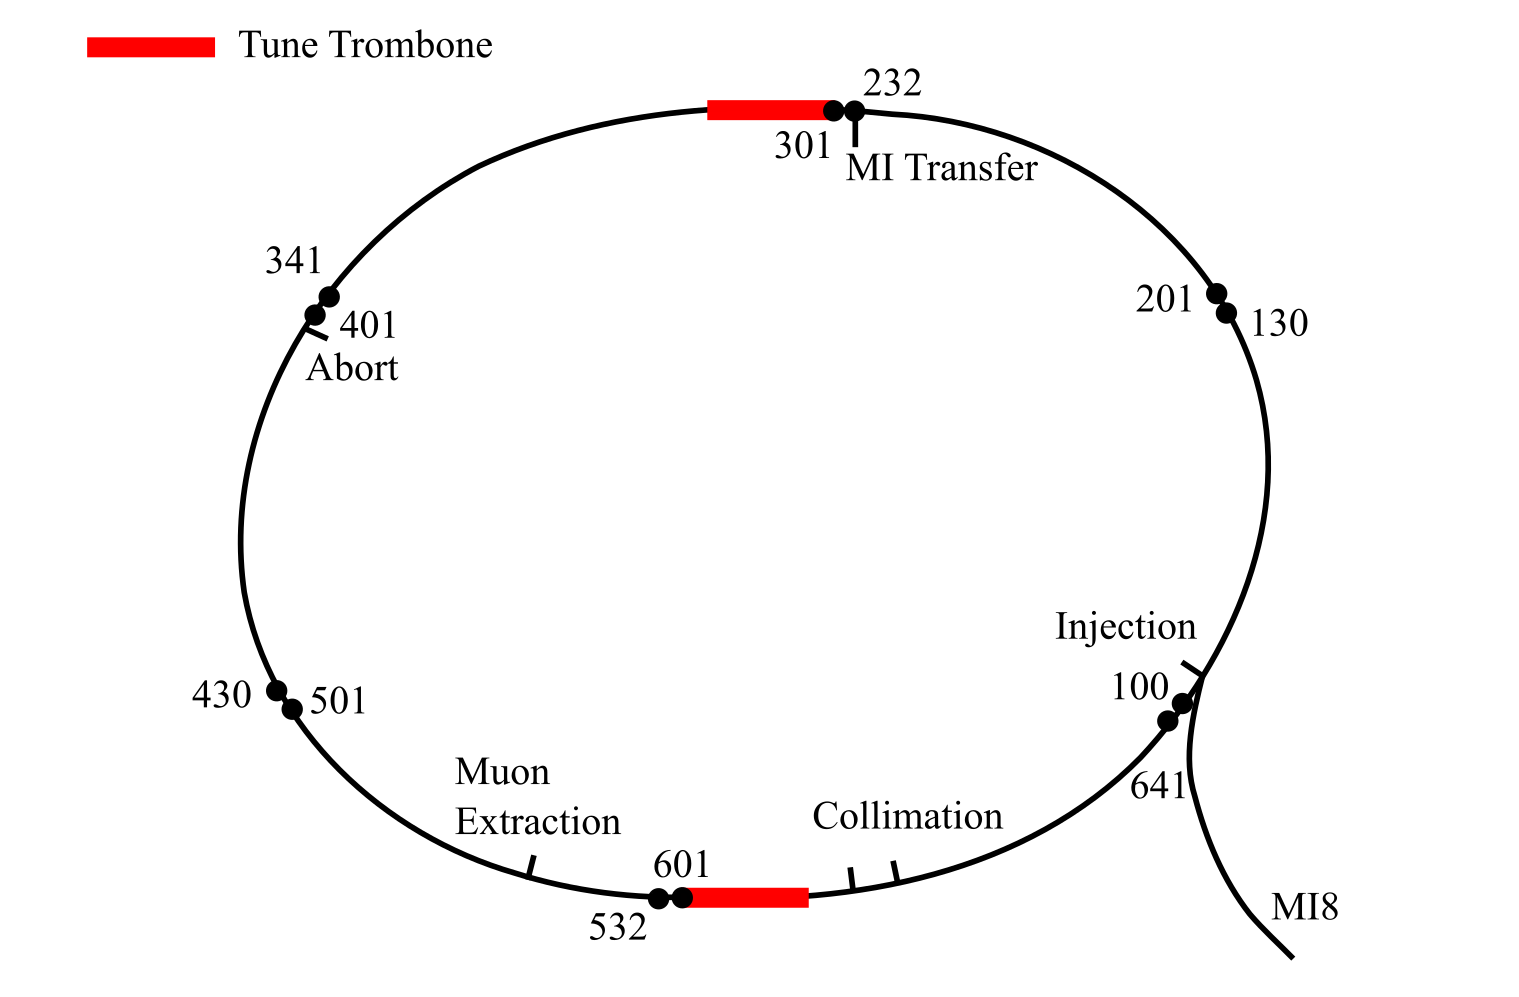
\includegraphics[width=\columnwidth]{chapter3/RRschematic.png}
   \caption{Schematic layout of the Recycler Ring and its corresponding sections. Original plot provided by R. Ainsworth, first published on Ref. \cite{rr1}.}
   \label{fig:rrschematic}
\end{figure}

\begin{table}[H]
\centering
\caption{Typical Recycler Ring properties for beam sent to NuMI}
\label{tab:rrparams}
\begin{tabular}{@{}ccc@{}}
\toprule
\textbf{Parameter}          & \textbf{Value}                             & \textbf{Unit} \\ \midrule
Circumference               & 3319.4                                     & m             \\
Momentum                    & 8.835                                      & GeV/c         \\
Revolution Period           & 11.1                                       & $\mu$s        \\
Revolution Frequency        & 90.1                                       & kHz        \\
RF Frequency                & 52.8                                       & MHz           \\
RF Voltage                  & 80                                         & kV            \\
Harmonic Number             & 588                                        &               \\
Synchrotron Tune            & 0.0028                                     &               \\
Slip Factor                 & -8.6 $\times$ 10$^{-3}$                    &               \\
Superperiodicity            & 2                                          &               \\
Horizontal Tune             & 25.43                                      &               \\
Vertical Tune               & 24.445                                     &               \\
Horizontal Chromaticity     & -6                                         &               \\
Vertical Chromaticity       & -7                                         &               \\
95\% Normalized Emittance   & 15                                         & $\pi$ mm mrad \\
95\% Longitudinal Emittance & 0.08                                       & eV s          \\
Intensity                   & $5\times10^{10}$                           & ppb           \\
                            & $8\times10^{10}$ (PIP-II)                  & ppb           \\
MI Ramp Time                & 1.2                                        & s             \\
                            & 1.133                                      & s             \\
                            & 1.067                                      & s             \\
Booster Frequency           & 15                                         & Hz            \\
                            & 20 (PIP-II)                                & Hz            \\ \bottomrule
\end{tabular}
\end{table}

\begin{figure}[H]
   \centering
   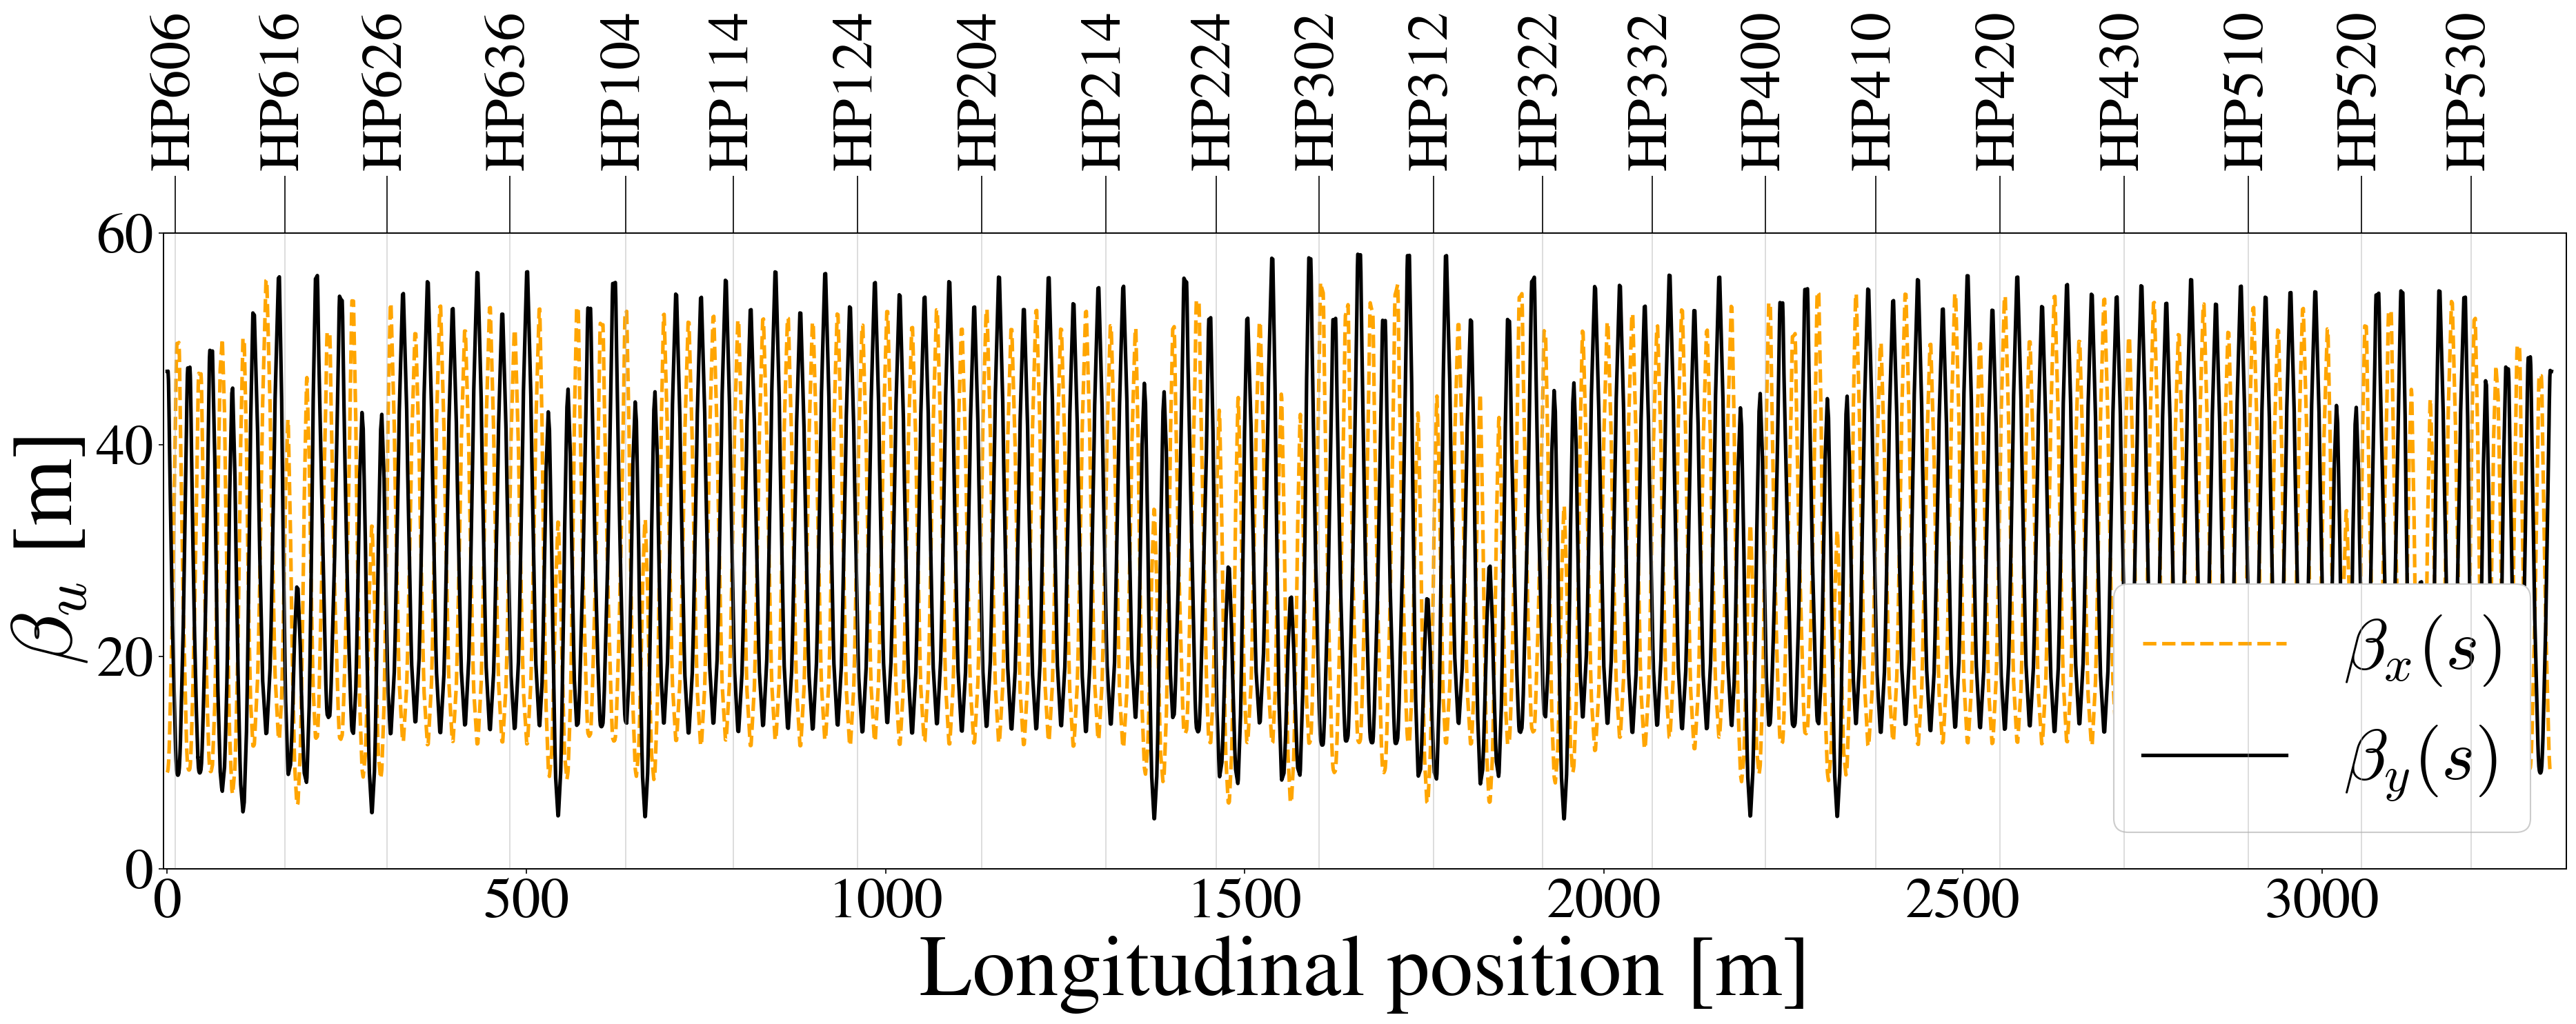
\includegraphics[width=\columnwidth]{chapter3/betas.png}
   \caption{Beta functions for the Recycler Ring lattice tuned to $Q_x=25.44$ and $Q_y=24.39$. Lattice functions calculated from lattice file using SYNERGIA.}
   \label{fig:rrbetas}
\end{figure}

\begin{equation}
   \label{eq:utotal}
   u(s) = u_{\beta}(s) + D_u(s) \delta
\end{equation}

\begin{figure}[H]
   \centering
   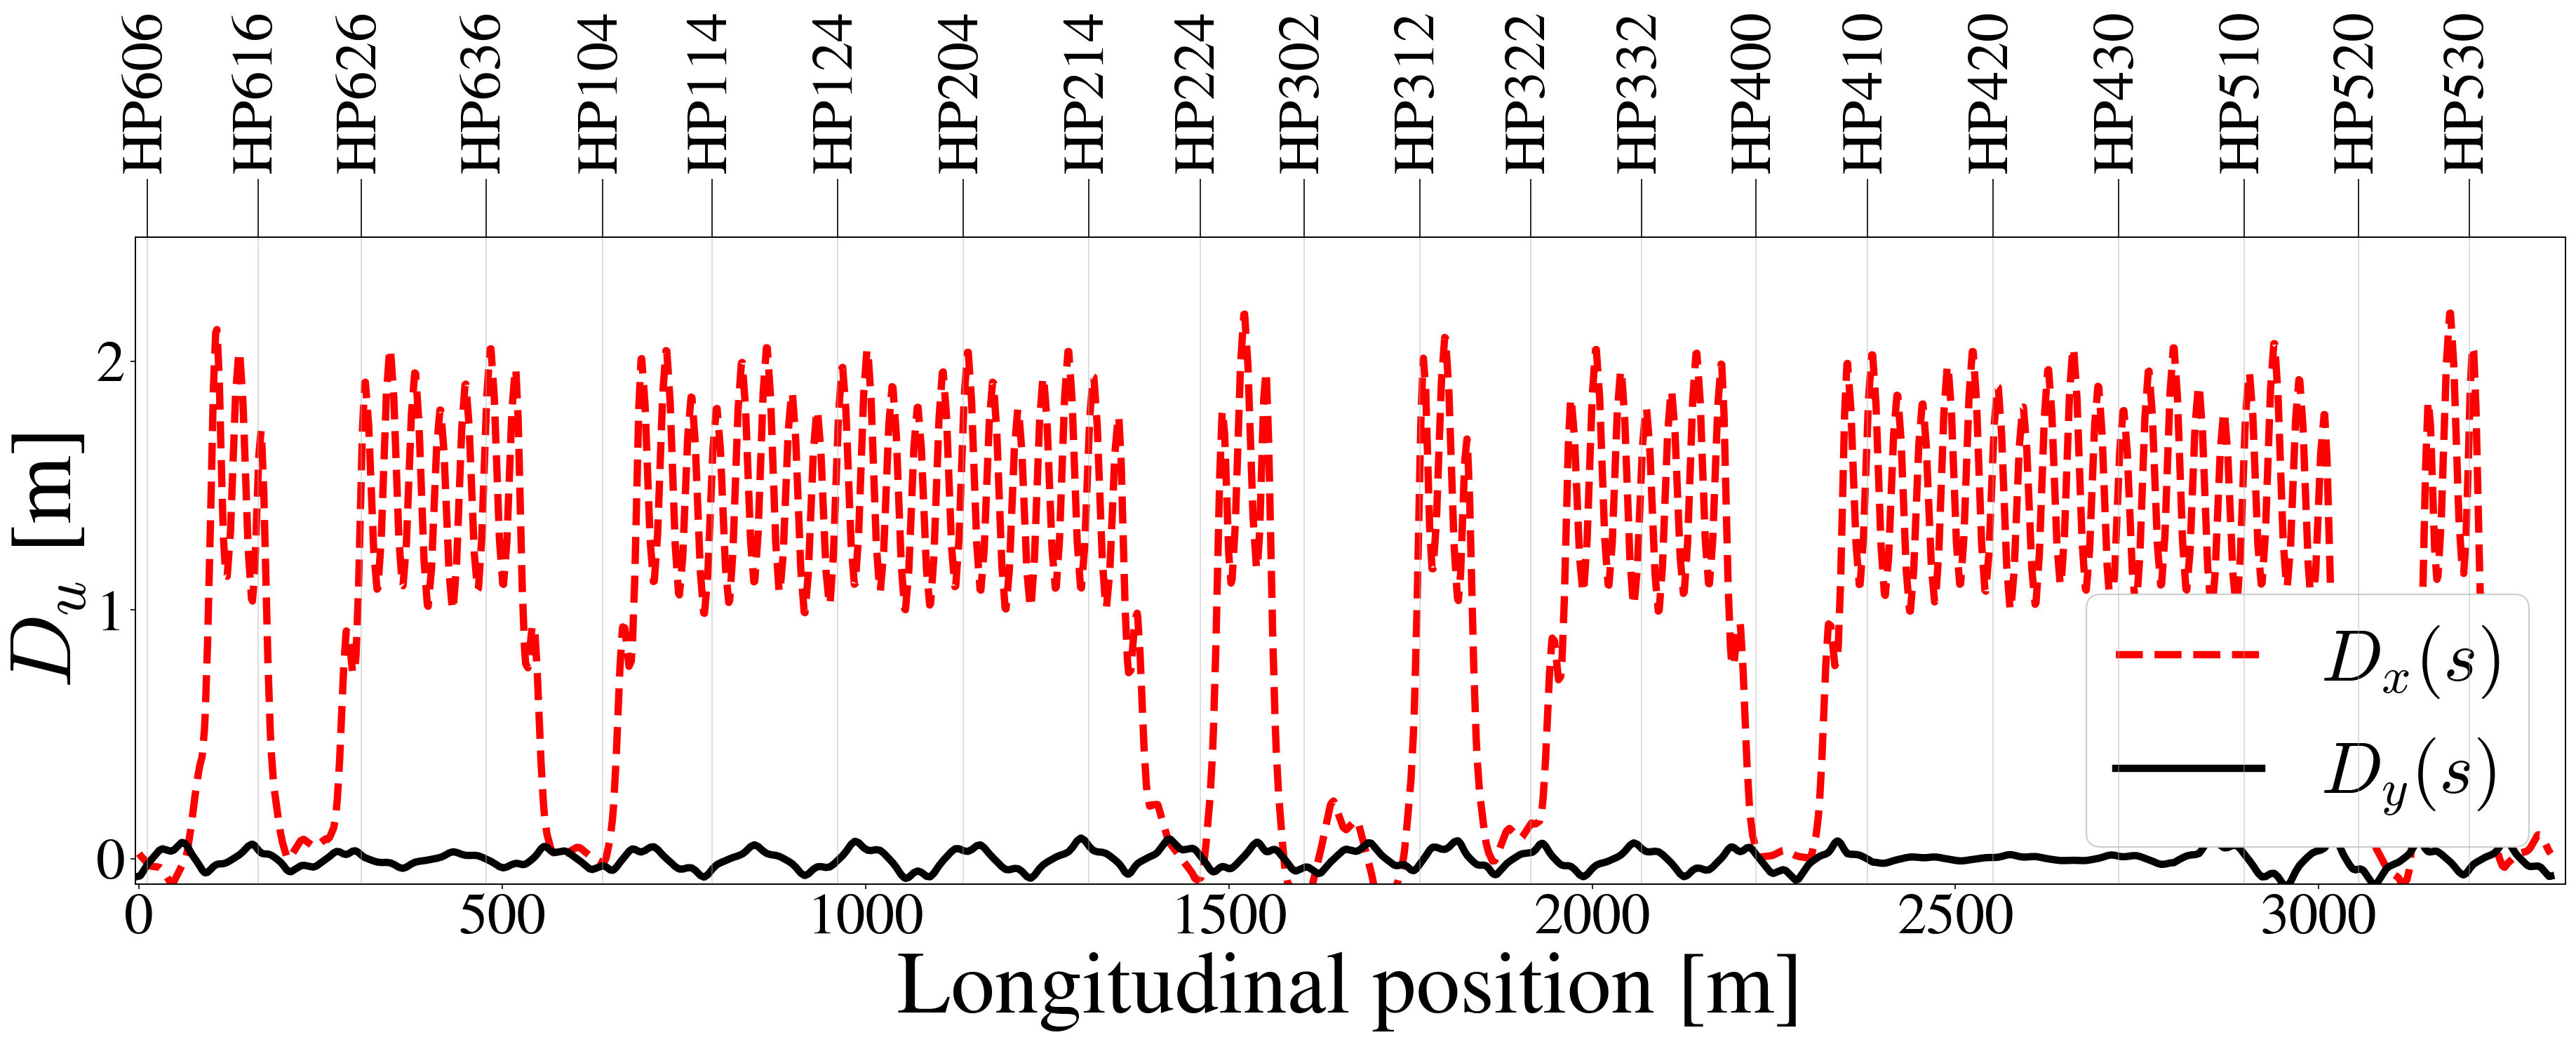
\includegraphics[width=\columnwidth]{chapter3/disps.png}
   \caption{Dispersion functions for the Recycler Ring lattice tuned to $Q_x=25.44$ and $Q_y=24.39$. Lattice functions calculated from lattice file using SYNERGIA.}
   \label{fig:rrdisps}
\end{figure}

\section{Tune Diagram and Resonances}

\begin{figure}[H]
   \centering
   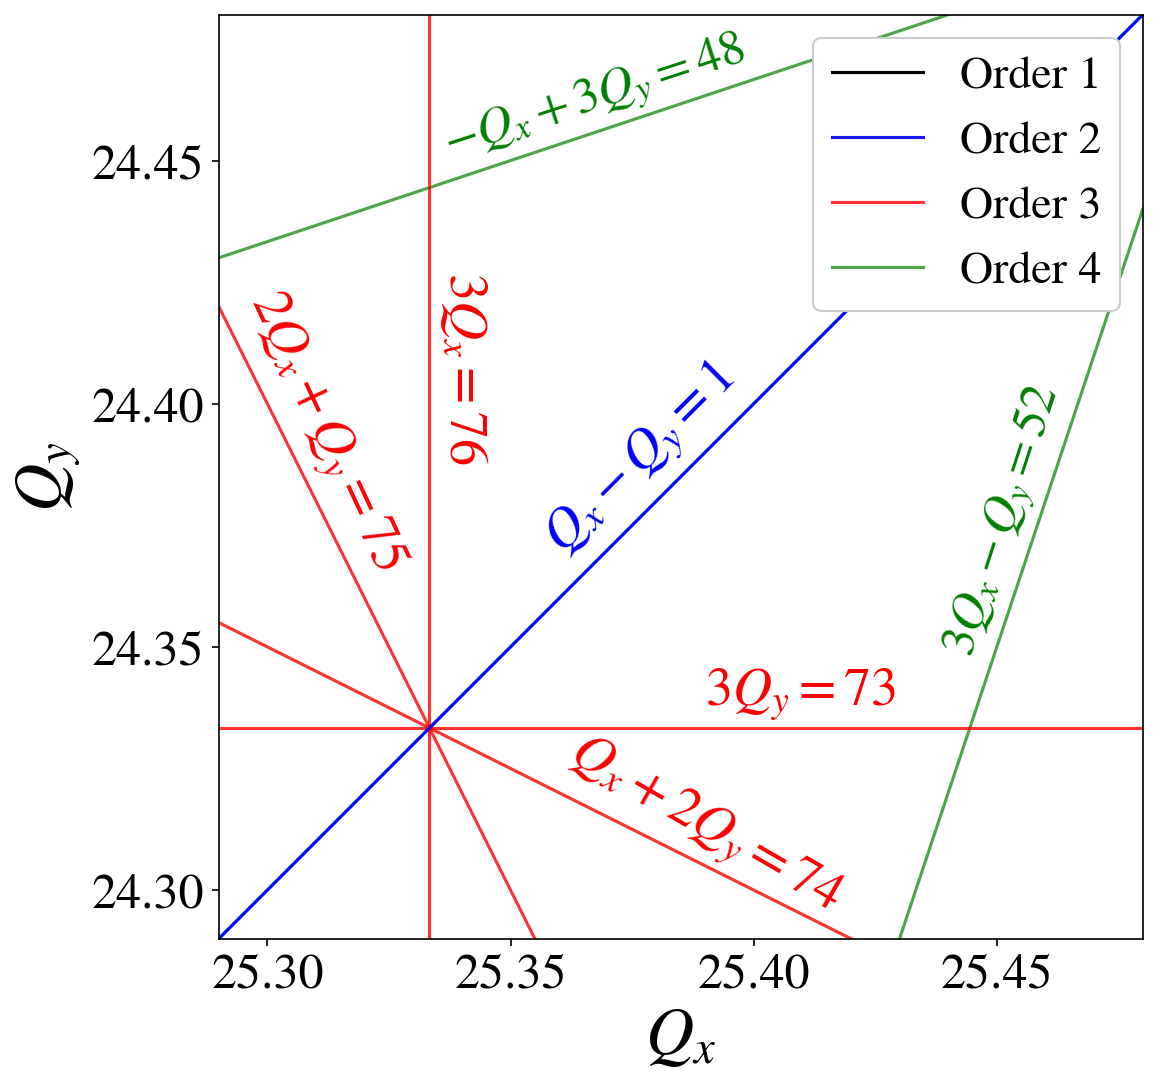
\includegraphics[width=\columnwidth]{chapter3/rrtd.png}
   \caption{Portion of the tune diagram enclosing the operational tunes of the Recycler Ring.}
   \label{fig:rrtd}
\end{figure}

\section{High Intensity and Tune Footprint}

\begin{figure}[H]
   \centering
   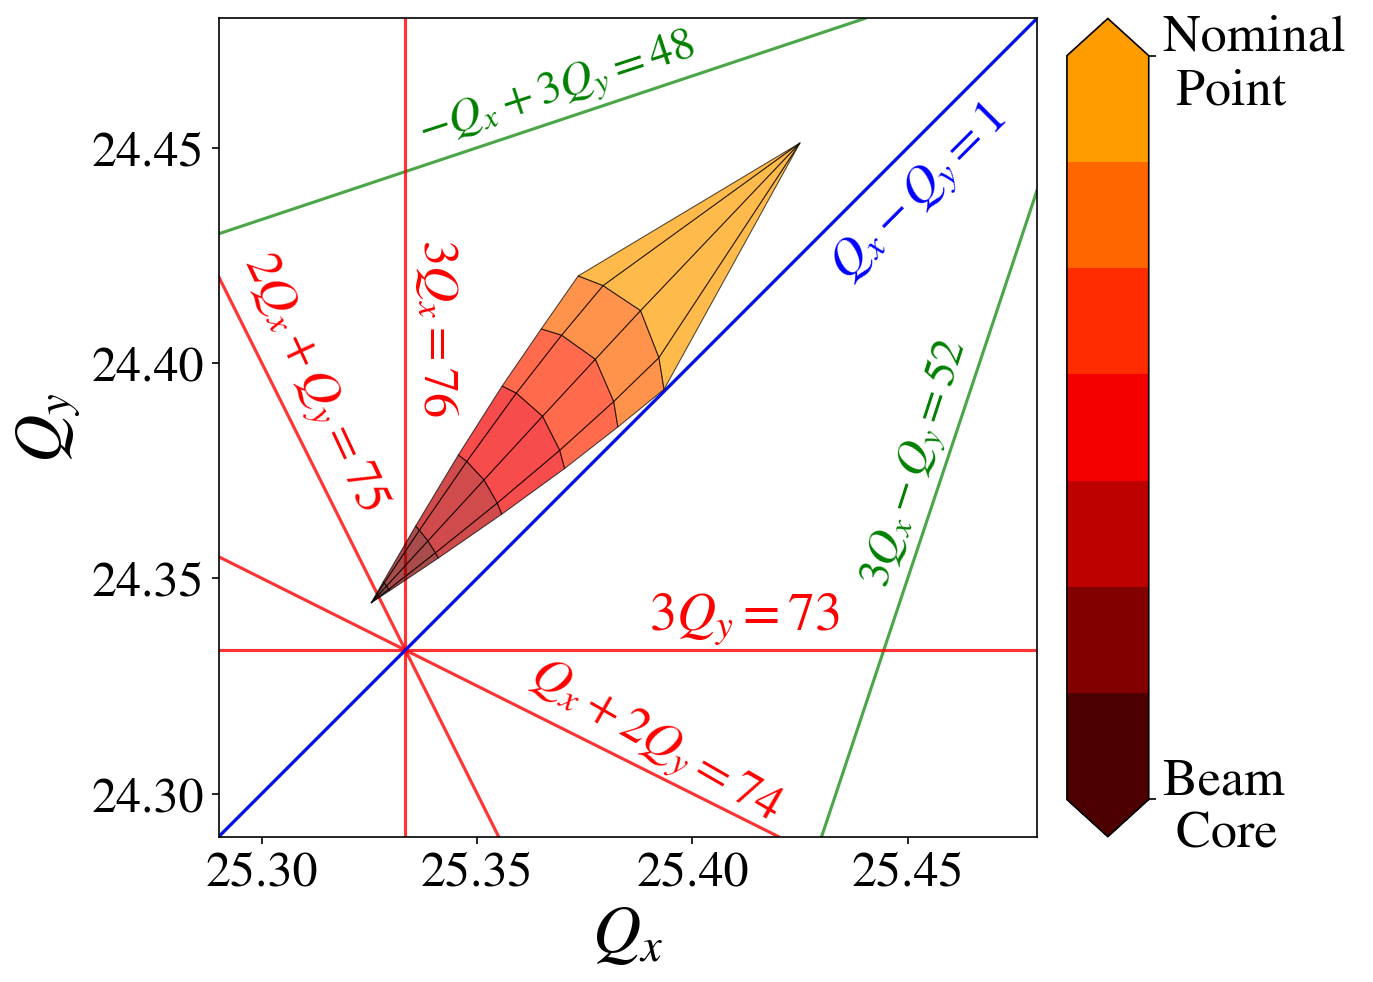
\includegraphics[width=\columnwidth]{chapter3/rrtdhigh.png}
   \caption{Approximate operational tune footprint at high intensities, i.e., 1e11 particles per bunch.}
   \label{fig:rrtdhigh}
\end{figure}

\section{Diagnostic Devices}

The Recycler Ring has two main diagnostic devices 

\begin{figure}[H]
   \centering
   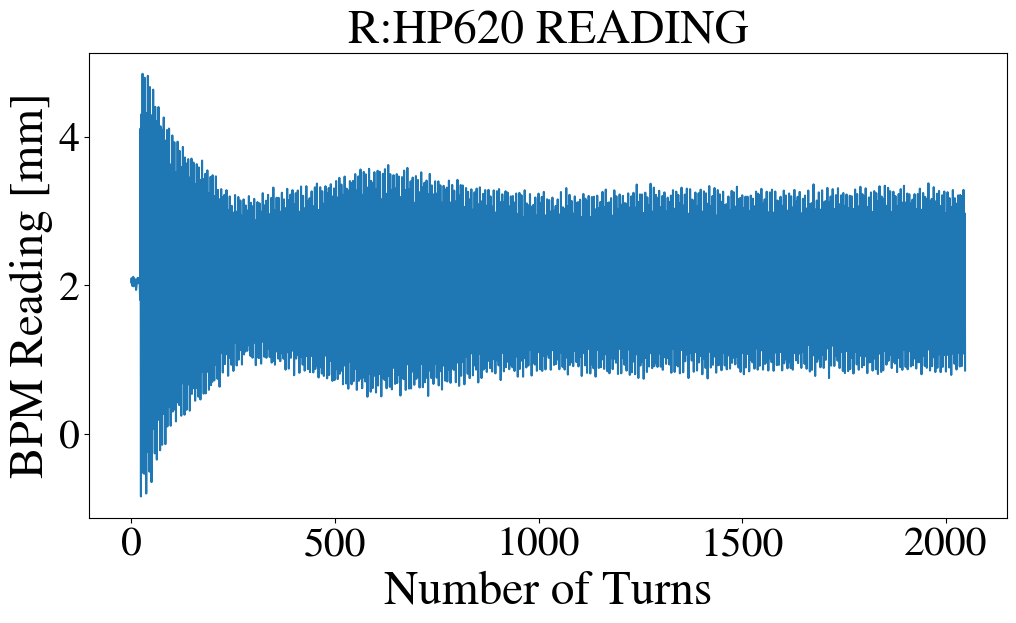
\includegraphics[width=\columnwidth]{chapter3/bpm_kick.png}
   \caption{BPM turn-by-turn data for an arbitrary kick at horizontal BPM R:HP620.}
   \label{fig:bpmkick}
\end{figure}

\begin{figure}[H]
   \centering
   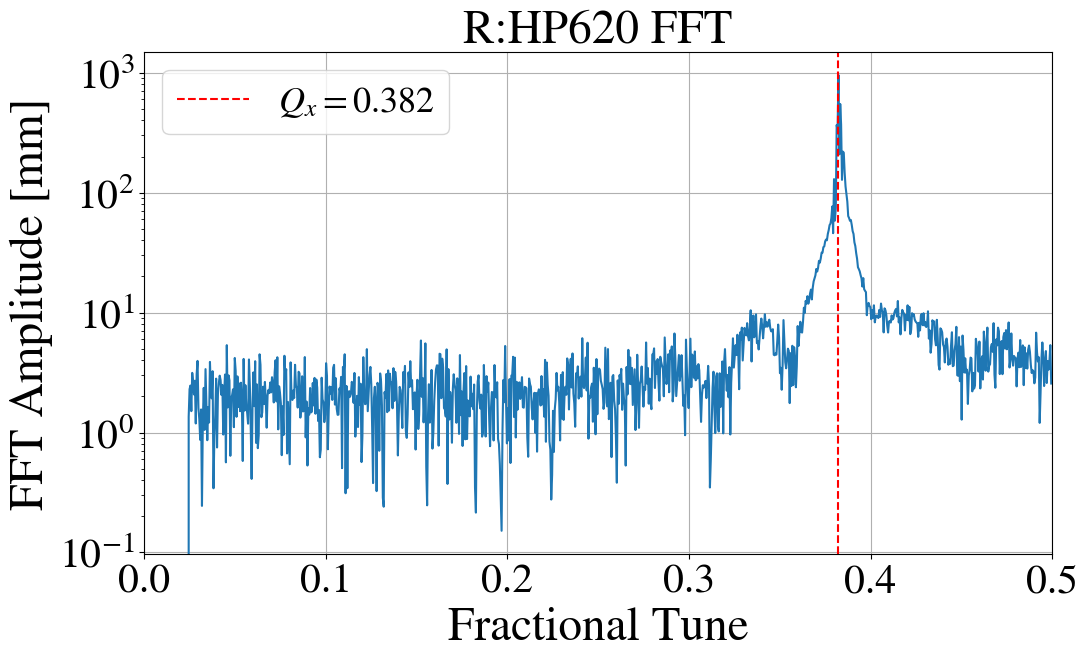
\includegraphics[width=\columnwidth]{chapter3/bpm_fft.png}
   \caption{Fast Fourier Transform amplitude for the turn-by-turn data presented in Fig. \ref{fig:bpmkick}.}
   \label{fig:bpmfft}
\end{figure}

\section{Elements for Resonance Compensation}

\begin{figure}[H]
   \centering
   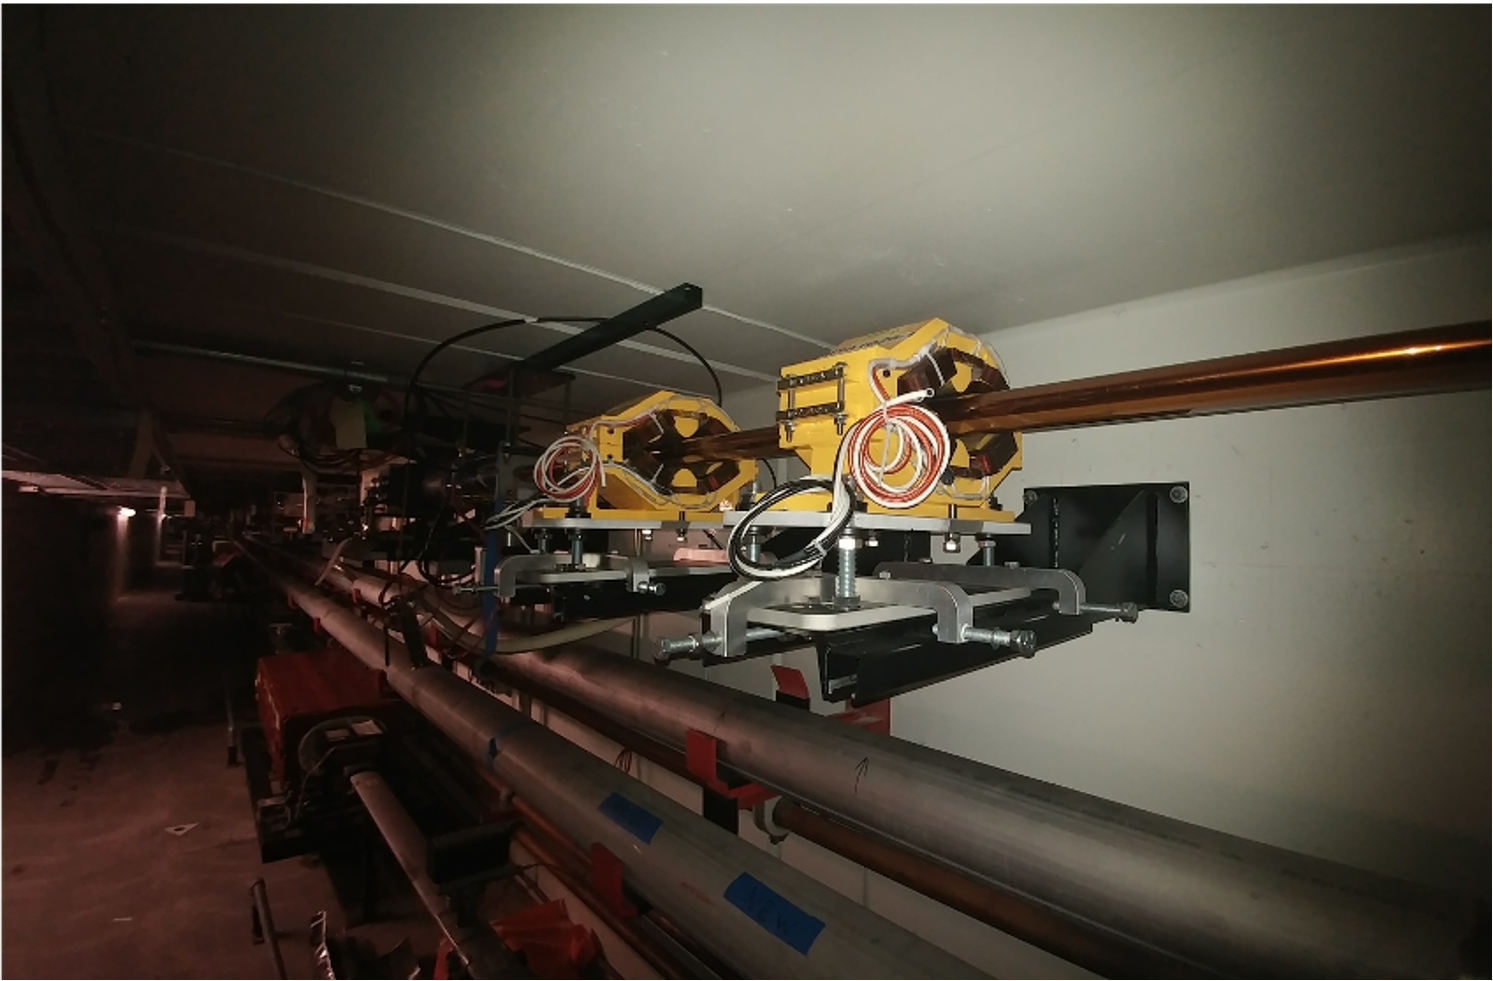
\includegraphics[width=\columnwidth]{chapter3/sextupoles.png}
   \caption{Picture of compensation sextupoles (yellow magnets on top) installed in the Recycler Ring.}
   \label{fig:sextupoles}
\end{figure}
\chapter{Compensation of Third-Order Resonances at Low Intensities}
\label{sec:ch4}

\section{Global RDTs and Lattice Model}

\section{Measurement of Third Order RDTs}

\section{Compensation of RDTs}

\section{Optimization of Compensation Currents}

\section{Experimental Verification of Compensation}

\subsection{Dynamic Loss Map}

\subsection{Static Tune Scans}

\chapter{Resonance Compensation Studies at the CERN Proton Synchrotron Booster}
\label{sec:ch5}

\section{General Description}
The Proton Synchrotron Booster (PSB) is the first circular accelerator in the CERN accelerator complex that ultimately leads to the LHC. Figure \ref{fig:cernac} shows the entire chain of accelerators at CERN, feeding a variety of physics experiments \cite{cernplot}. Following the successful implementation of the LHC Injectors Upgrade (LIU) \cite{liu}, the PSB receives $H^-$ ion beam coming from the Linac4 at an energy of 160 MeV. Interestingly enough, the PSB is not just one ring, but rather four synchrotron rings stacked on top of each other. This is to counteract space charge effects which are largest at low energy machines. Once the ion beam enters the PSB rings, the electrons are stripped off with a carbon foil and proton beam is achieved \cite{psbstrip}. The proton beam is then accelerated from an energy of 160 MeV to 2 GeV. The beam from the four rings gets merged together and then gets injected to the Proton Synchrotron (PS). This is true for LHC-type beams, nevertheless, the PSB can also accelerate lead ions and deliver to heavy ion experiments like ISOLDE \cite{foteini1}.   \cite{foteini2} 

\begin{figure}[H]
    \centering
    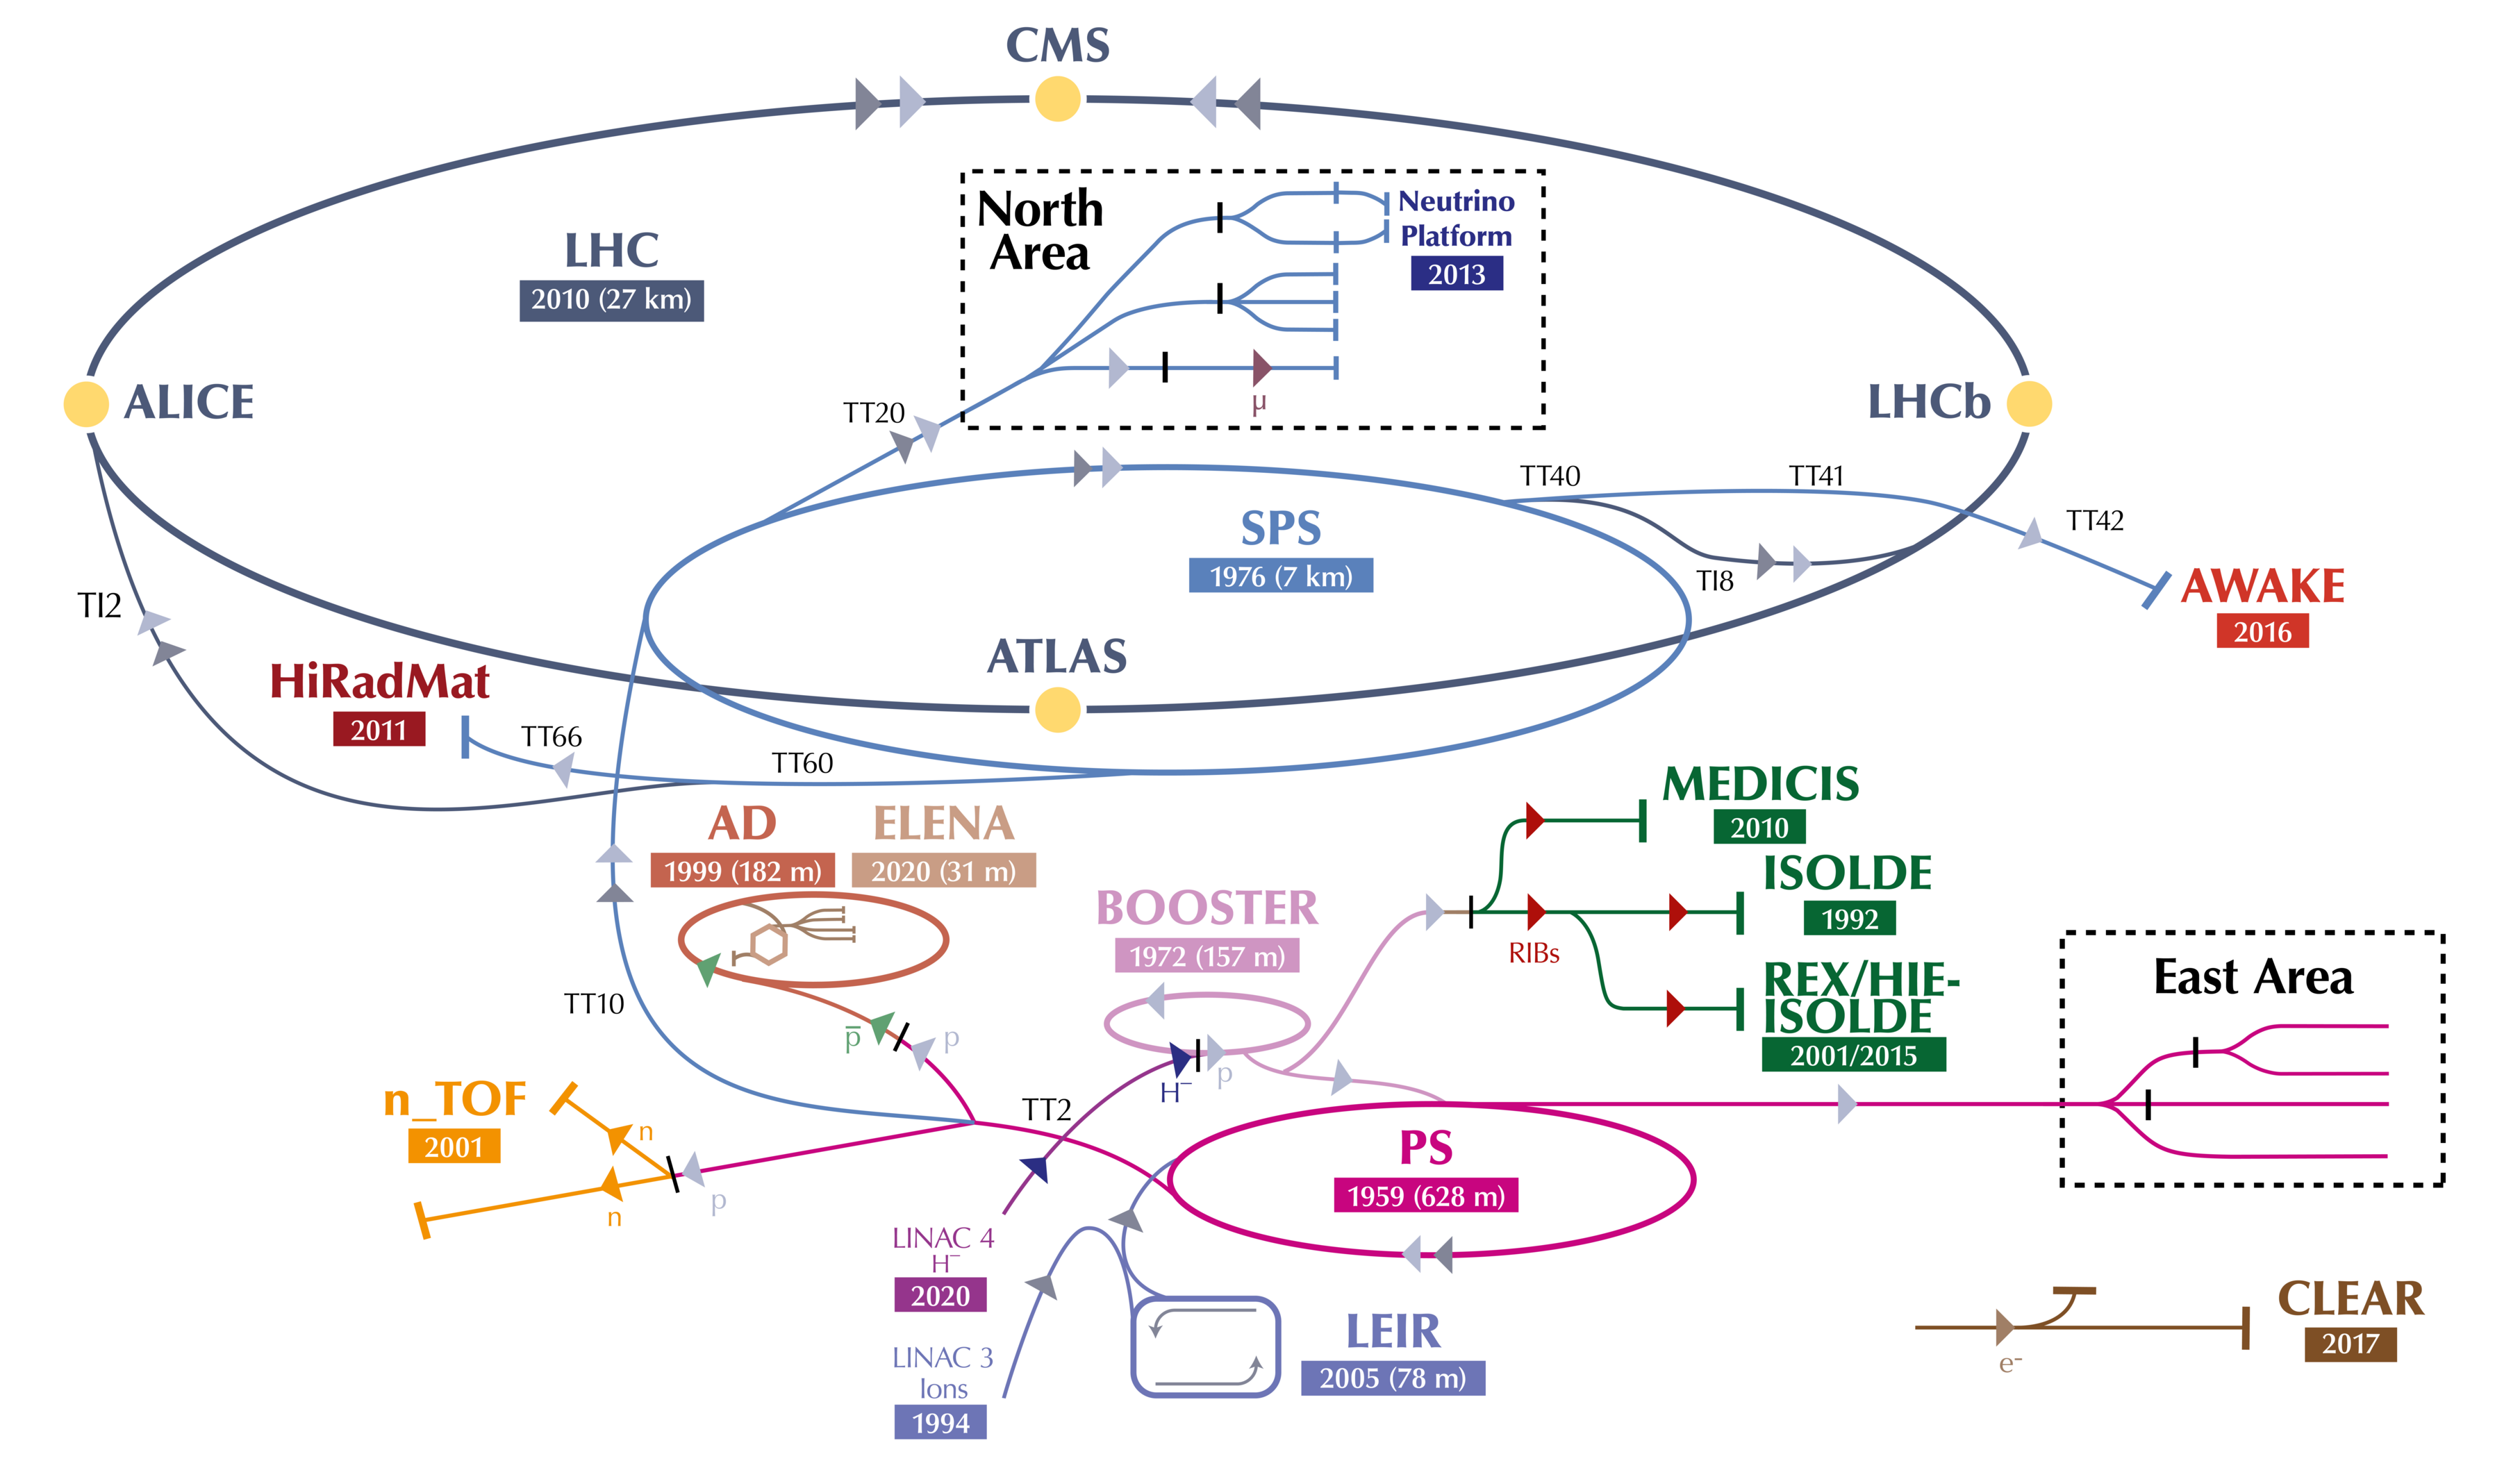
\includegraphics[width=\linewidth]{chapter5/CERN_AC.png}
    \caption{A graphic overview of all accelerators in operation at CERN as of 2022. Original image taken from Ref. \cite{cernplot}. This file is licensed under the Creative Commons Attribution 4.0 International license.}
    \label{fig:cernac}
 \end{figure}

\section{Tune Diagram and Operation}

\section{Optimization Algorithms for Resonance Compensation}

\section{Experimental Verification of Compensation}

\chapter{High Intensity Studies}
\label{sec:ch6}

\section{Global RDTs and Intensity-Dependent Effects}
\cite{mionrr}
\section{Space Charge Tune Shift}

\begin{equation}
    \Delta \nu_{sc}=\frac{-3 N r_0 R S}{4 \sigma_z M \beta \gamma ^2 \varepsilon_{N,95\%}}    
\end{equation}

\section{Measurement of Tune Spread}

% \newpage
% \begin{figure}[H]
%     \centering
%     \includegraphics[height=\textheight,keepaspectratio]{chapter6/scts_measure.png}
%     \caption{Tune spread.}
%     \label{fig:dynamictunespread}
% \end{figure}
% \newpage

\begin{figure}[H]
    \centering
    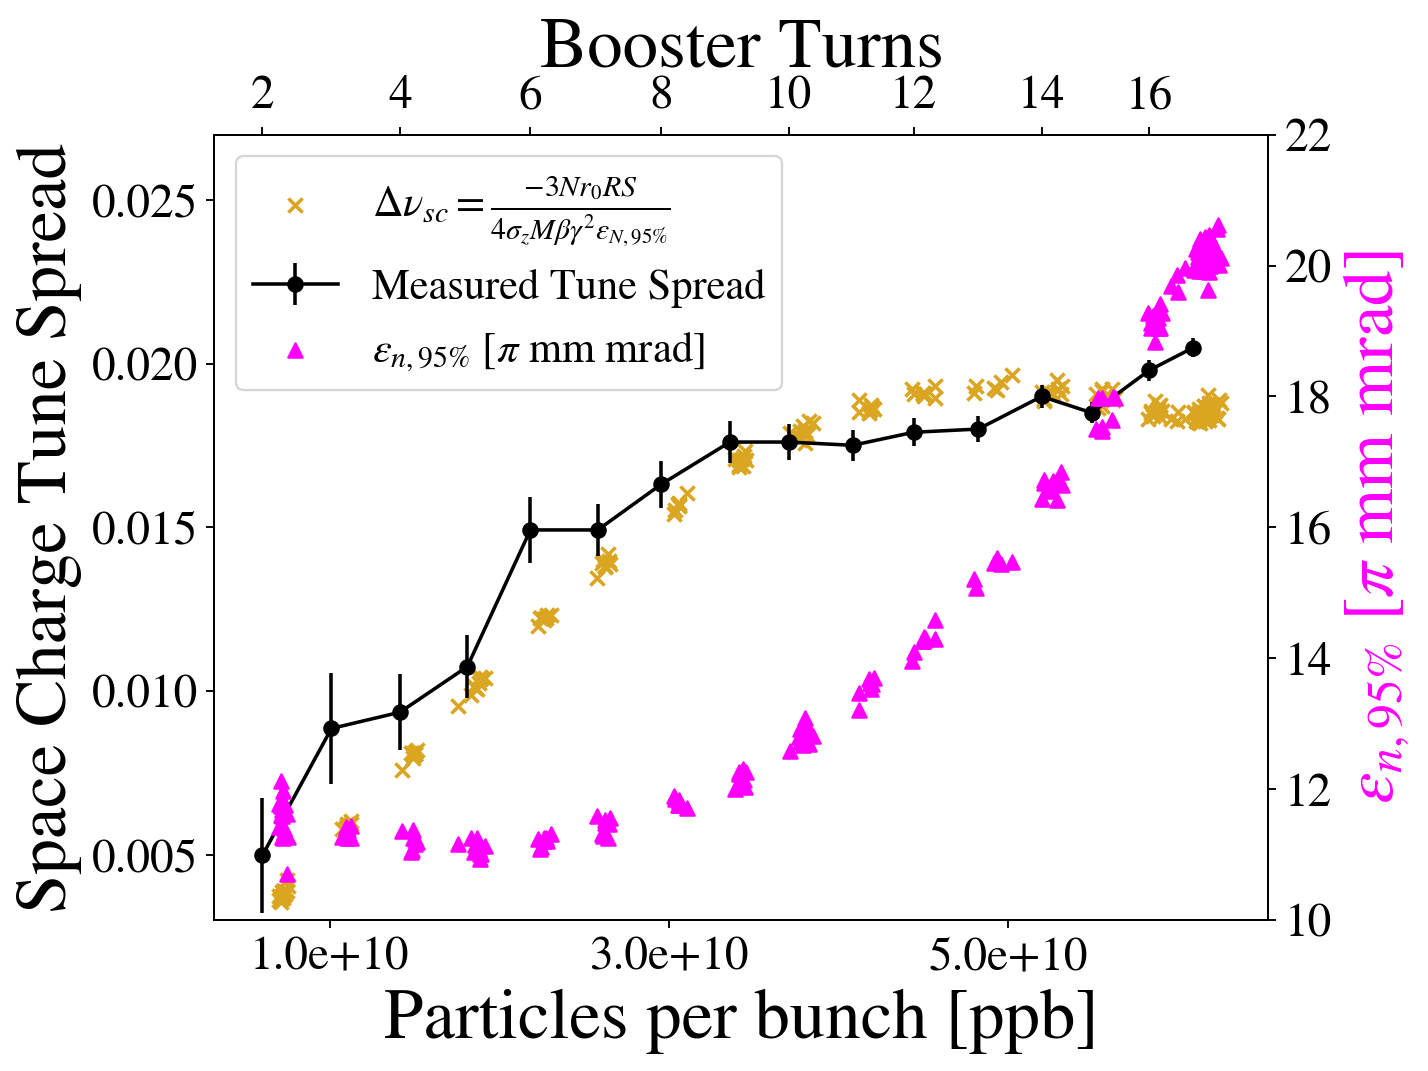
\includegraphics[width=\columnwidth]{chapter6/tune_spread.png}
    \caption{Measurement of tune spread.}
    \label{fig:tunespread}
\end{figure}

\section{Static Tune Scans at Different Intensities}

\section{Effect of Transverse Dampers}

\begin{figure}[H]
    \centering
    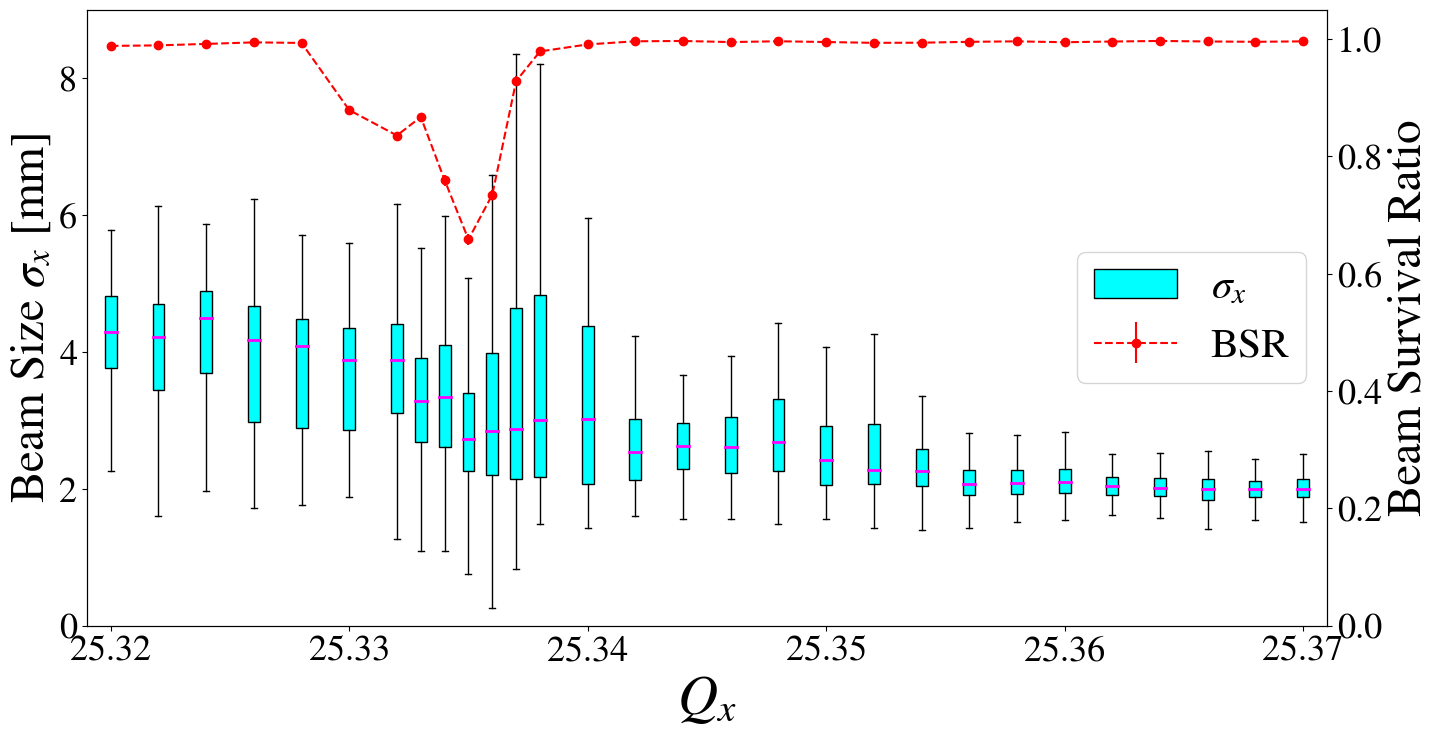
\includegraphics[width=\columnwidth]{chapter6/static2turns_ipm_dampersON.png}
    \caption{Static tune scan with beam survival ratio and IPM data box plots with $3Q_x$ compensation, transverse dampers ON and 2 Booster Turns of equivalent intensity.}
    \label{fig:static2_dampersON}
\end{figure}

\begin{figure}[H]
    \centering
    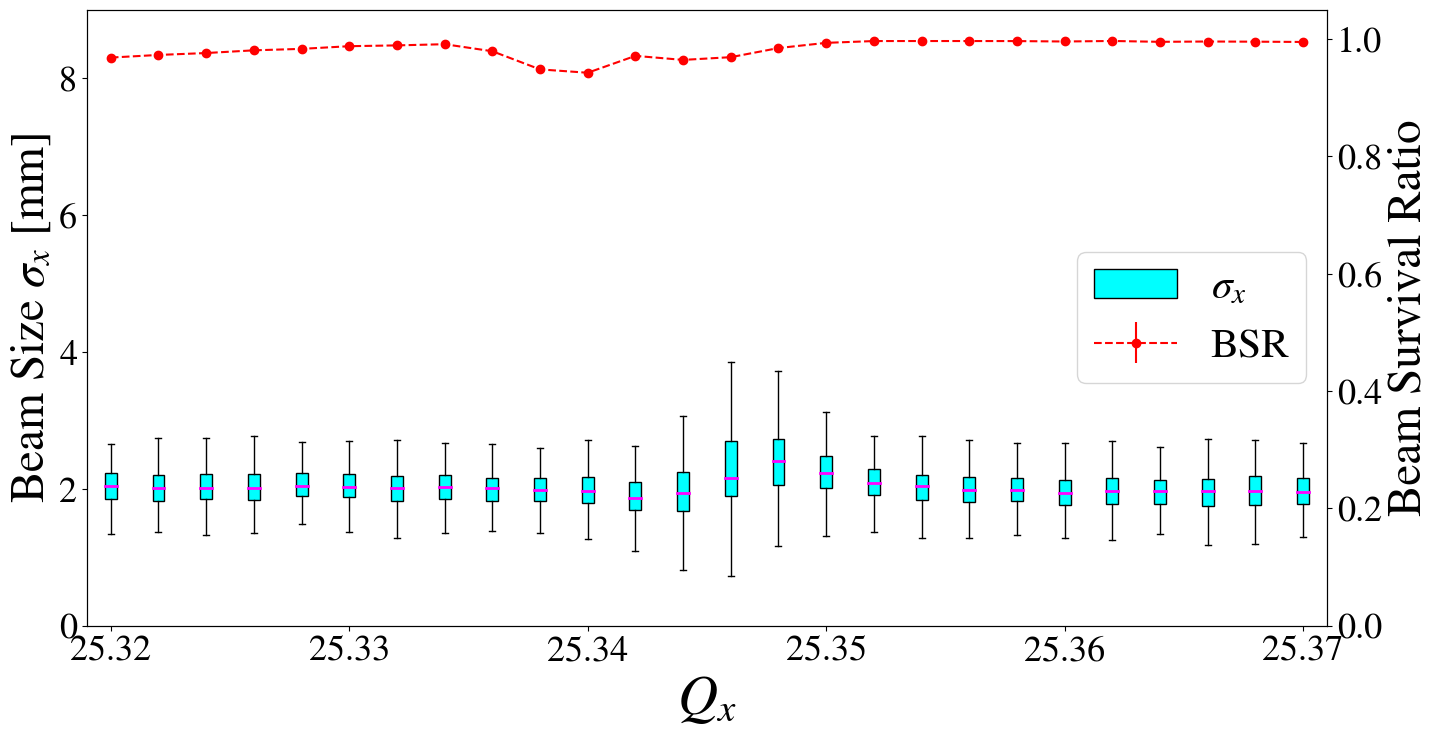
\includegraphics[width=\columnwidth]{chapter6/static2turns_ipm_dampersOFF.png}
    \caption{Static tune scan with beam survival ratio and IPM data box plots with $3Q_x$ compensation, transverse dampers OFF and 2 Booster Turns of equivalent intensity.}
    \label{fig:static2_dampersOFF}
\end{figure}
\chapter{Conclusions and Future Work}
\label{sec:ch7}

The work shown throughout this document can also be found in Refs. \cite{cris1,cris2, cris3}. This section reports on the conclusions and future work stemming from this thesis.

\section{Conclusions}

\subsection{RDTs and Resonance Compensation}

The measurement and subsequent cancellation of RDTs was investigated in depth in Ch. \ref{sec:ch4}. It was shown that third order RDTs in the Recycler Ring can be measured and, afterwards, cancelled with the compensation sextupoles in place. Furthermore, optimization procedures have been developed in order to have this compensation   

\subsection{Physics-Informed vs. Optimization-Based Compensation}

Chapters \ref{sec:ch4} and \ref{sec:ch5} showed two different approaches to the same problem of resonance compensation. The first one performed at the Fermilab Recycler Ring showed how to implement the response matrix approach, which can be traced to some underlying physics principles. On the other hand, Ch. \ref{sec:ch5} shows how to implement numerical optimization algorithms for compensating multiple resonance lines at the CERN PS Booster. Nevertheless, this last approach had no direct physics input. The distinction between a physics-informed approach and a numerical-optimization approach summarizes the differences between both chapters. The 

\subsection{High-Intensity Resonance Compensation}

For current operations of the Fermilab Accelerator Complex, the third-order resonance compensation scheme developed in this work will not have an effect on reducing losses in the Recycler Ring. The current tune spreads in the RR are not large enough for the third order resonances to be specially harmful to operations. The beam coming out of Booster grows exponentially with the beam intensity, as it was shown in Fig. \ref{fig:tunespread}. Thus, saturating the tune spread at values close to 0.02---not particularly large. The losses in the Recycler Ring are purely emittance-dominated for current operations. They are not related to space charge effects. Nonetheless, the resonance compensation scheme still is beneficial to operations at high intensities. This is if the operational tune is moved closer to the third order resonance lines, which is not suggested.  

\subsection{Transverse Dampers and High-Intensity Compensation}

Section \ref{sec:ch6dampers} showed how the transverse dampers have an effect on the resonance compensation scheme. Figure \ref{fig:dampers7} reinforces this statement by showing the beam survival ratio at a high intensity of 4.5e10 ppb without compensation and dampers on(bare machine), with compensation and dampers on, and with compensation and dampers off. Ultimately, the dampers degrade the quality of the compensation. In particular, when turned off, the overall beam survival ratio increases. The configuration of the dampers---gain and phase of feedback---has been optimized away from the resonance lines. When the tunes are set close to the third order resonance lines, the dampers settings will create beam size growth. They are not optimized to run in this region, and will cause harmful effects on the beam, even with the resonance compensation scheme enabled.

\begin{figure}[H]
    \centering
    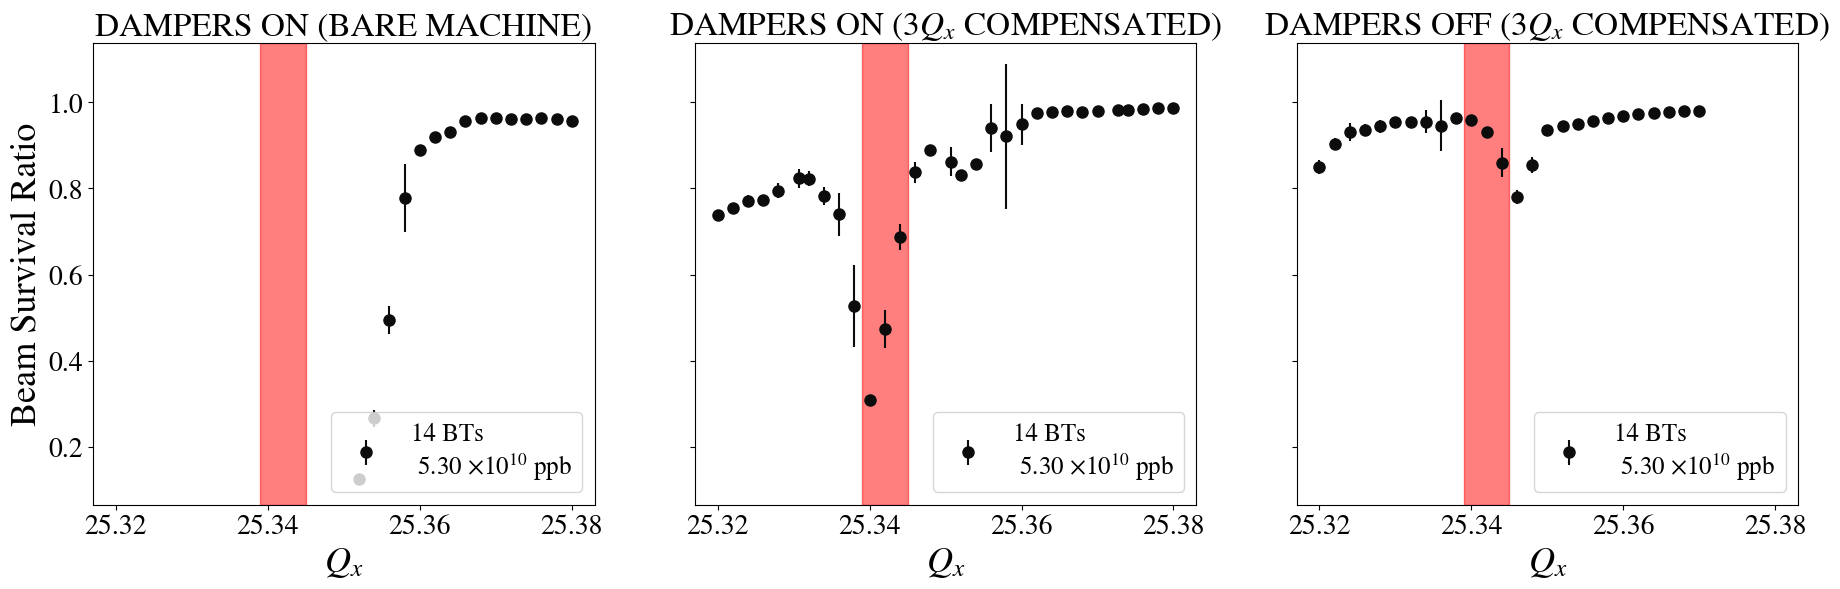
\includegraphics[width=\columnwidth]{chapter7/dampers_config.png}
    \caption{Transverse damper effect on resonance compensation for bare machine + dampers ON, $3Q_x$ compensated + dampers ON, and $3Q_x$ compensated + dampers OFF configuration. The red band corresponds to the $3Q_x$ stop band at an intensity of 0.5 ppb with dampers ON.}
    \label{fig:dampers7}
\end{figure}

\section{Future Work}

\subsection{Verification of Newly-Installed Sextupoles}

Section \ref{sec:compensate} explained the motivation behind installing additional sextupoles that would bring down that currents needed to compensate $3Q_x=76$ and $Q_x+ 2Q_y = 74$. Subsequently, Sec. \ref{sec:addsexts} explained the procedure used in order to pin down the new locations for two new compensation sextupoles. There is still future work to be done regarding the commissioning and connection of the new 620 sextupoles. The sextupoles and their power supplies need to be interfaced with ACNET. Furthermore, the resonance compensation enhancement still needs to verified by means of performing an RDT scan. Specifically, the response matrix coefficients corresponding to these new sextupoles need to be measured and calculated. All of this, following the procedure outlined in Secs. \ref{sec:rdtmeasure} and \ref{sec:compensate}. Figure \ref{fig:new620sexts} shows a picture of the newly installed sextupoles.

\begin{figure}[H]
    \centering
    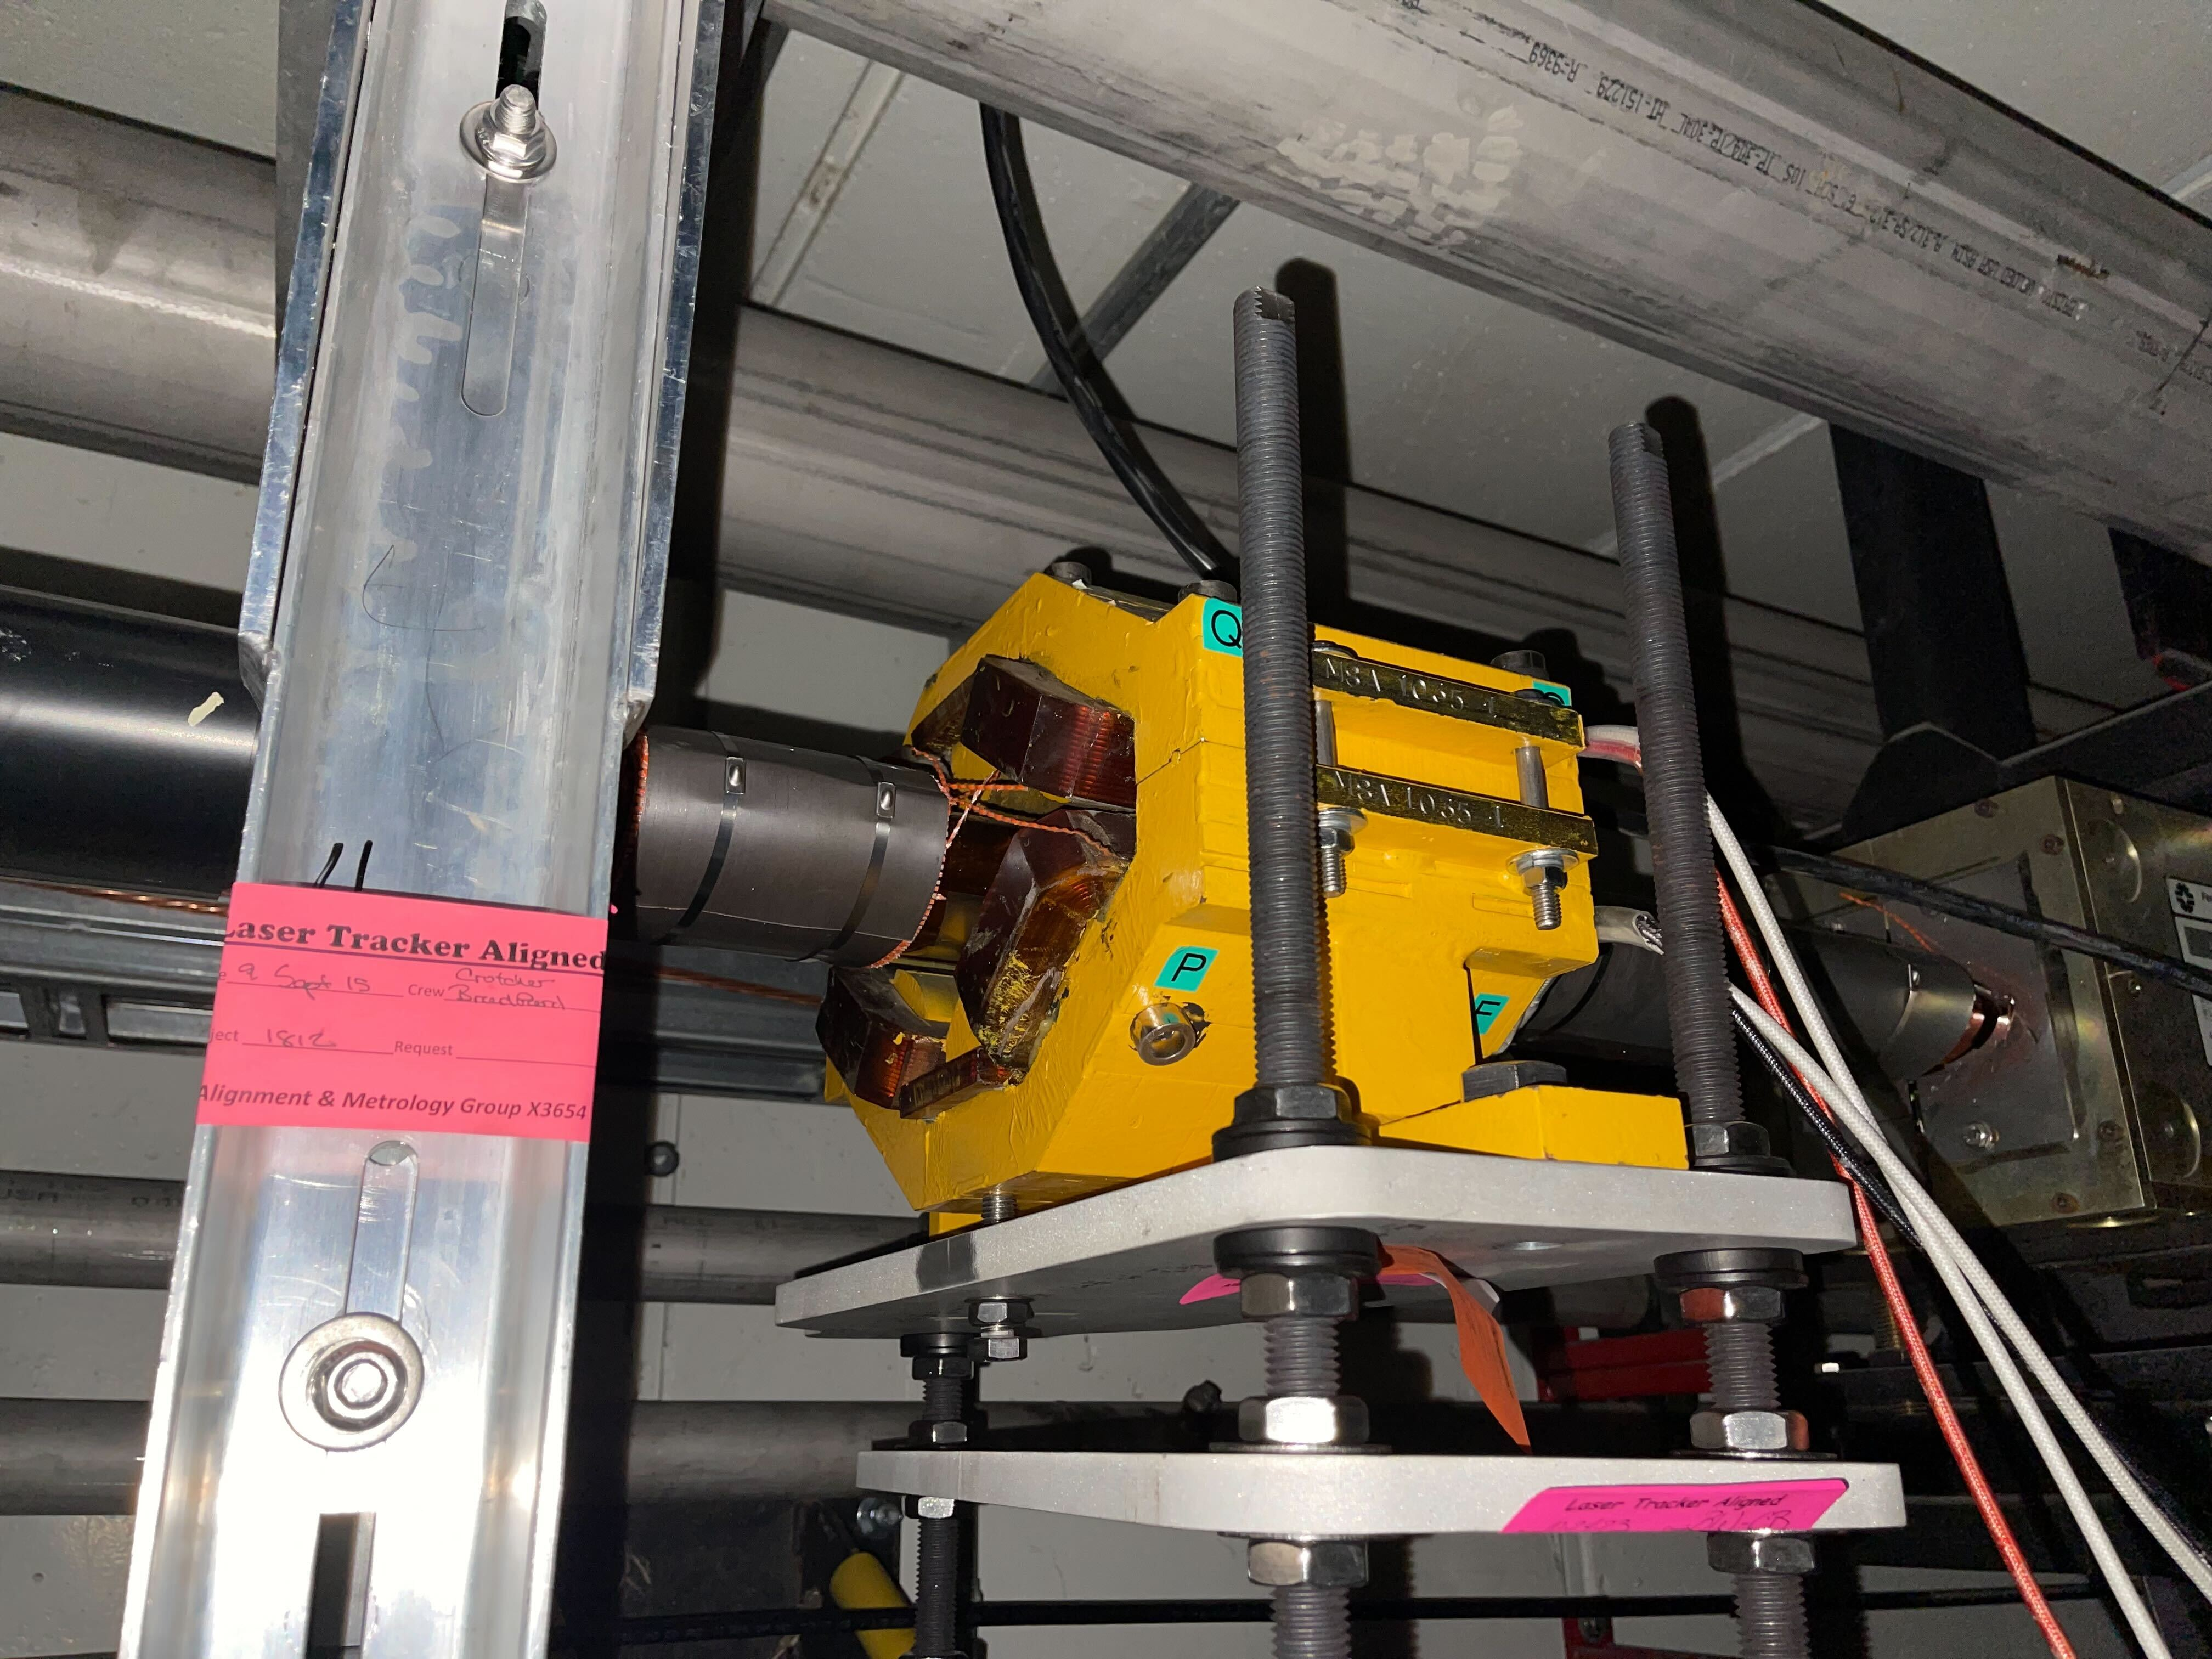
\includegraphics[width=\columnwidth]{chapter7/620_sext.jpg}
    \caption{Newly installed compensation sextupoles in the 620 section.}
    \label{fig:new620sexts}
\end{figure}

\subsection{Resonances and Transverse Dampers at High Intensities}

It was shown in Sec. \ref{sec:ch6dampers} that the transverse dampers in the Recycler Ring can interact with betatron resonance lines depending on their configuration. It would be interesting to perform experiments with the configuration of these dampers in order to fully characterize these effects. Furthermore, it would also be interesting to use the dampers as anti-dampers in order to sustain betatron oscillations. With this configuration, one could perform tune measurements, and perhaps evaluate this alternative method to measure RDTs. This would be similar to having an AC dipole installed in the Recycler.  

\subsection{Effect of MI Ramp on RDTs}

The ultimate objective of this work is to have this resonance compensation scheme fully characterized in order to incorporate it into high intensity operations. Nevertheless, there is one additional factor that has been identified to also play a role in this effort. This one stems from the fact that the Main Injector and the Recycler Ring share the same tunnel. It has been shown that the acceleration ramp changes the beam dynamics inside the Recycler Ring. In particular, it introduces orbit distortions and tune shifts depending on the position of the ramp \cite{mionrr}. There is an ongoing effort in order to characterize any higher order magnetic effect from the MI to RR, e.g., any sextupole term that is being introduced by the MI acceleration ramp. The first results have shown that the compensation currents change depending on the location of the study event with respect to the MI acceleration ramp. Therefore, in the future, the resonance compensation described hereinabove should be modified to accommodate this effect to be fully operational.

\subsection{Limits of Resonance Compensation}

\subsection{Space Charge RDTs}

Equation \ref{eq:hfinal} shows how the lattice elements and the space charge potential drive betatron resonances. It would be interesting to explore further how to measure space charge resonance driving terms (SCRDTs) and their effect on the operation of the Recycler Ring. Without taking into account any collective instabilities, the ultimate limit of the Recycler Ring will be dictated by how strong these third order lines become in the space-charge dominated regime. The current future of the Main Injector and Recycler Ring lies in high-intensity beam. As the space charge potential grows for the Fermilab beams, it is important to quantify all effects from high intensity operation---being SCRDTs one of them.

\printbibliography
%\chapter{Your first chapter}
%
% If you have pages that must appear in landscape mode, use the [lscape] documentclass option
% and enclose the pages in a {landscape} environment.
%\clearpage\pagestyle{lscape} % first clear the page and change the pagestyle
%\begin{landscape}
%
% your landscape table(s) or figure(s) here
%
%\end{landscape}
%\pagestyle{plain} % remember to change the pagestyle back to plain
%
%
% Your bibliography command here 
% e.g. \bibliography{your-bib-file}) if using natbib
% e.g. \printbibliography if using biblatex
%
% Remember that although the bibliography is single spaced, there needs to
% be a blank line between entries. This is set by your bibliography package
% If you are using natbib it is \bibsep; if using biblatex it's \bibitemsep
% These are set automatically by the class if you are using these packages
%
% If you need per-chapter bibliographies, you need to use the [chapterbib]
% class option and you would use \makebibliographypage before each
% chapter level bibliography and then the relevant bibliography command
% You should not use the \backmatter command 
%
% If you have appendices, they would go here.  
% If you only have one appendix it will look like this: (comment this out if you have no appendices)
% \begin{appendices}
% \chapter{\label{sec:app1}Lie Algebra Methods for Accelerator Physics in 2D using MATHEMATICA}
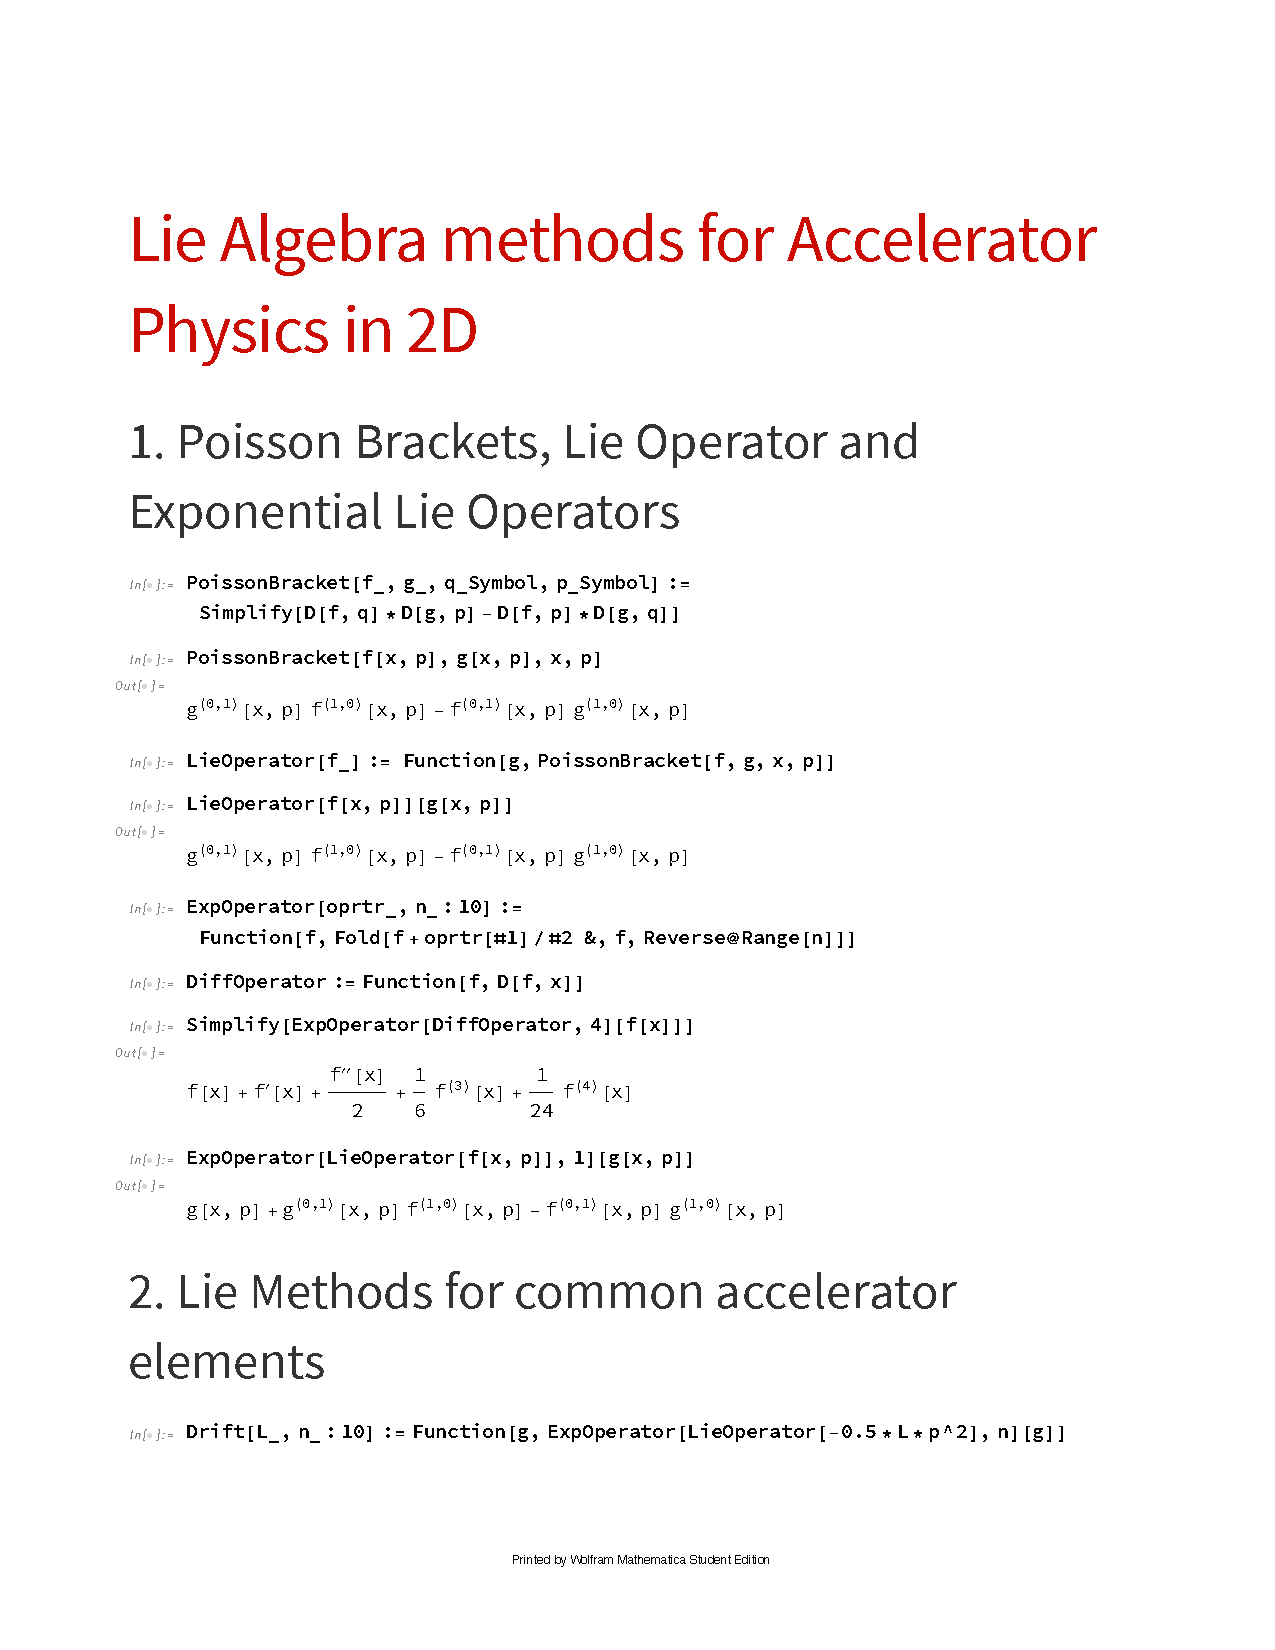
\includepdf[pages=-]{lie2D.pdf}
% \chapter{\label{sec:app2}Lie Algebra Methods for Accelerator Physics in 4D using MATHEMATICA}
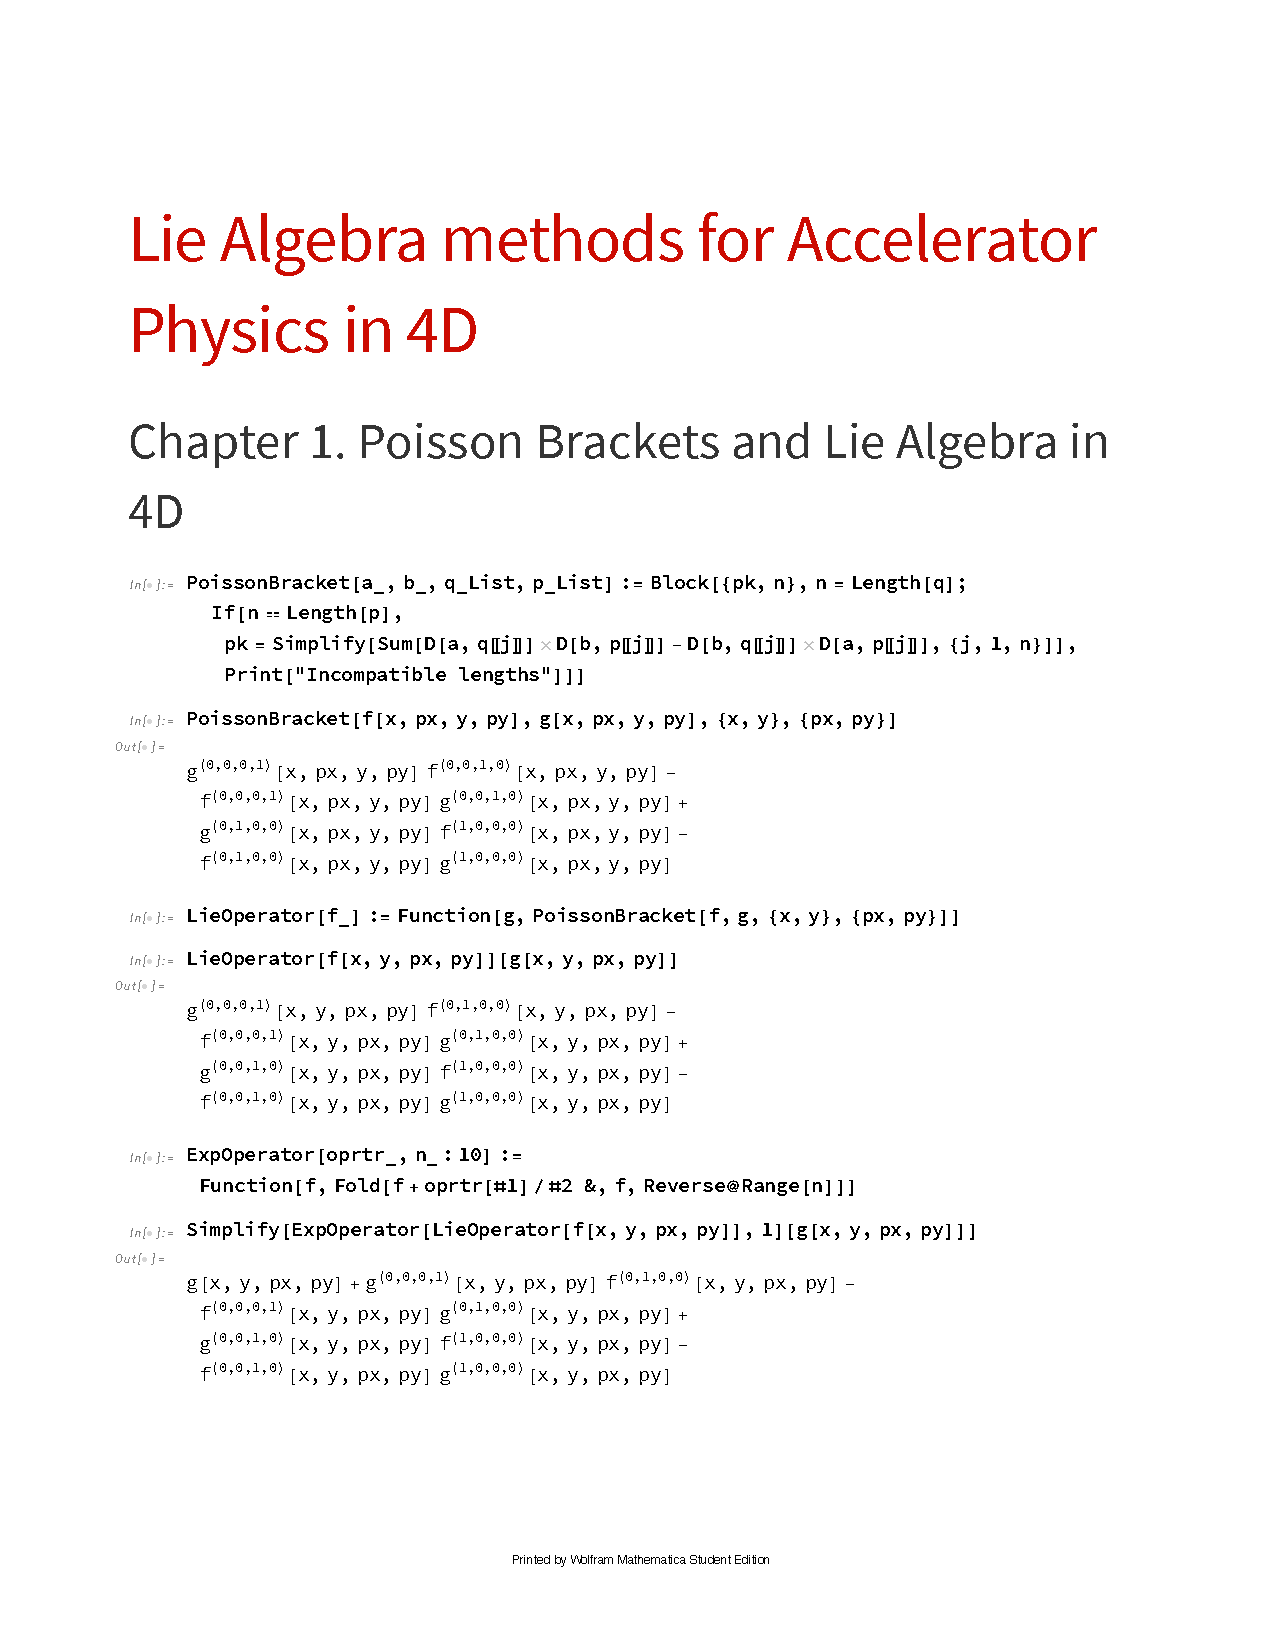
\includepdf[pages=-]{lie4D.pdf}
% \end{appendices}
%
%
% If you have more than one appendix, you need to use 
%   \begin{appendices}
%   \chapter{First appendix}
%   \chapter{Second appendix}
%   \end{appendices}
%
% If each chapter has its own set of appendices, then load the class with the [chapterapp] option
% and put your {appendix} or {appendices} environments at the end of each chapter.
%
%
% Even though it is very unintuitive, per-chapter appendices are STILL \chapter commands
% in your document!  If you use \section it will not work properly.
% 
% You should not use the \backmatter command 
\end{document}

